% UG project example file, February 2022 Do not change the first two lines of
% code, except you may delete "logo," if causing problems. Understand any
% problems and seek approval before assuming it's ok to remove ugcheck.
\documentclass[logo,bsc,singlespacing,parskip]{infthesis}
\usepackage{ugcheck}
\newcommand{\todo}{\textbf{?} }
\usepackage{color,soul}
% \usepackage{hyperref}
\usepackage{graphicx}
\usepackage{array}
\usepackage{xcolor}
\usepackage{soul}
\usepackage{booktabs}
\usepackage{fancyvrb}
\usepackage{relsize}
\usepackage{float}
\usepackage[hidelinks]{hyperref}

\newcommand{\sigfpe}{\texttt{SIGFPE}}
\newcommand{\dthalfi}{\texttt{int10\char`_t}}
\newcommand{\dtshort}{\texttt{int16\char`_t}}
\newcommand{\dtint}{\texttt{int32\char`_t}}
\newcommand{\dtlong}{\texttt{int64\char`_t}}
\newcommand{\dthalf}{\texttt{half}}
\newcommand{\dtfloat}{\texttt{float}}
\newcommand{\dtfloati}{\texttt{int23\char`_t}}
\newcommand{\dtdouble}{\texttt{double}}
\newcommand{\feinexact}{\texttt{FE\char`_INEXACT}}
\newcommand{\feinvalid}{\texttt{FE\char`_INVALID}}
\newcommand{\mxcsr}{\texttt{mxcsr}}
\newcommand{\pivot}{\texttt{pivot}}
\newcommand{\mca}{\texttt{llvm-mca}}
\newcommand{\exegesis}{\texttt{llvm-exegesis}}
\newcommand{\xmm}{\texttt{XMM}}
\newcommand{\ymm}{\texttt{YMM}}
\newcommand{\zmm}{\texttt{ZMM}}

\newenvironment{VerbatimCompact}
  {\vspace*{-2.5mm}\VerbatimEnvironment
   \par\Verbatim}
  {\endVerbatim\vspace*{-2.4mm}}


\newcolumntype{V}[1]{>{\topsep=0pt\@minipagetrue}p{#1}<{\vspace{-\baselineskip}}}
\makeatother
\newcommand{\command}[1]{\texttt{\string#1}}

\newcommand{\hlc}[2][yellow]{{%
    \colorlet{foo}{#1}%
    \sethlcolor{foo}\hl{#2}}%
}

\newcolumntype{L}[1]{>{\raggedright\let\newline\\\arraybackslash\hspace{0pt}}m{#1}}
\newcolumntype{C}[1]{>{\centering\let\newline\\\arraybackslash\hspace{0pt}}m{#1}}
\newcolumntype{R}[1]{>{\raggedleft\let\newline\\\arraybackslash\hspace{0pt}}m{#1}}

\newenvironment{compactlist}
{ \begin{enumerate}
    \setlength{\itemsep}{0pt}
    \setlength{\parskip}{0pt}
    \setlength{\parsep}{0pt}     
}
{ \end{enumerate} } 

% Include any packages you need below, but don't include any that change the page
% layout or style of the dissertation. By including the ugcheck package above,
% you should catch most accidental changes of page layout though.

\usepackage{microtype} % recommended, but you can remove if it causes problems

\begin{document}
\begin{preliminary}

\title{Fast \pivot{} Function for Presburger Library through Vectorization and
Integer Arithmetic in FPU}

\author{Zhou Qi}

% CHOOSE YOUR DEGREE a):
% please leave just one of the following un-commented
% \course{Artificial Intelligence}
%\course{Artificial Intelligence and Computer Science}
%\course{Artificial Intelligence and Mathematics}
%\course{Artificial Intelligence and Software Engineering}
%\course{Cognitive Science}
\course{Computer Science}
%\course{Computer Science and Management Science}
%\course{Computer Science and Mathematics}
%\course{Computer Science and Physics}
%\course{Software Engineering}
%\course{Master of Informatics} % MInf students

% CHOOSE YOUR DEGREE b):
% please leave just one of the following un-commented
%\project{MInf Project (Part 1) Report}  % 4th year MInf students
%\project{MInf Project (Part 2) Report}  % 5th year MInf students
\project{4th Year Project Report}        % all other UG4 students


\date{\today}

\abstract{
\label{sec:abstract}

This report presents a fast implementation for the core function \pivot{} of a
math library in MLIR by performing vectorized integer arithmetics in
FPU. The hot loop of the \pivot{} function performs overflow-checked
multiplication and addition on each element of an input matrix of low dimension
and mostly small value items. MLIR's upstream uses element-wise
transprecision, from \dtlong{} to \texttt{LargeInteger}. 
This can be improved if hardware resources are utilized effectively, by taking
advantage of SIMD, and reducing the bit width for every element. 
The current approach cannot be automatically vectorized by compiler,
and \dtlong{} has a much larger bit width than what is
typically used for most of the items in the matrix.
Additionally, extra arithmetics are required to perform overflow checking 
for integers, resulting in significant overhead. 
This report ``innovates'' the
\dtfloati{}
% \footnote{This is not really a innovation. It it a common
% technique on GPUs because often they are more capable on floating points than
% integers. See Section \ref{sec:introduction} for more history and detail. }
datatype, a 23-bit integer datatype created from the 23-bit mantissa of a
32-bit floating point, to address these issues. 
\texttt{int23\_t} overflow can be captured as floating point imprecision by a
status register, making overflow awareness almost free.  
On a selected 30-row by 20-column representative input matrix, the runtime of
is reduced from 550 ns to 26 ns, achieving 20 times speedup.

% \hl{TODO:Question: mention int16 here?}

% \hl{TODO:Question: 16-column is not representative!}

% \hl{Reminder: we don't use int16 for (1) bad compatibility (2) it is not significanlty faster than float}

}

\maketitle

\newenvironment{ethics}
   {\begin{frontenv}{Research Ethics Approval}{\LARGE}}
   {\end{frontenv}\newpage}

\begin{ethics}

This project was planned in accordance with the Informatics Research
Ethics policy. It did not involve any aspects that required approval
from the Informatics Research Ethics committee.

\standarddeclaration
\end{ethics}


\begin{acknowledgements}
% First and foremost, I would like to express my deepest gratitude to my
% supervisor, Tobias Grosser, for his unwavering support, guidance, and
% encouragement throughout the course of this research. His extensive knowledge,
% valuable insights, and patience have been instrumental in shaping my academic
% and personal growth.

% I am also immensely grateful to Arjun Pitchanathan, a fellow Ph.D. student under
% the supervision of Tobias Grosser, for his invaluable assistance and
% collaboration. His expertise, constructive feedback, and willingness to share
% his knowledge have significantly contributed to the progress and quality of this
% work.

% Furthermore, I would like to acknowledge the generous contributions from Marisa
% Kirisame, Emanon, gjz010, and lyzh, whose insightful comments, technical
% support, and camaraderie have enriched my research experience. Their shared
% wisdom and passion for the subject matter have made this journey both enjoyable
% and rewarding.

% Finally, I am thankful to all my friends, colleagues, and family members who
% have provided me with the emotional support and encouragement needed to complete
% this paper. Their unwavering belief in my abilities has been a source of
% strength and motivation throughout this challenging process.

\end{acknowledgements}


\tableofcontents
\end{preliminary}


\chapter{Introduction}
\label{sec:introduction}

MLIR, Multi-Level Intermediate Representation, is a infrastructure for building
reusable and extensible compilers. Its aim is to reduce fragmentation in domain
specific languages and heterogeneous hardwares~\cite{mlir}. Its Presburger
library provides polyhedral compilation techniques to make dependence analysis
and loop optimization~\cite{mliraffine} and cache modeling~\cite{CacheModel}.
Presburger arithmetics involves determining whether conjunction of linear
arithmetic constraints is satisfiable~\cite{SMLPPA}, and can be solved using the
simplex method of linear programming, with its core function \pivot{} is the
main performance bottleneck~\cite{FPL1}. 

The \texttt{pivot} function involves two multiplication and one addition
operation on every element in a matrix. Notably, the input matrices for this
library tend to exhibit characteristics of small values and low dimensionality.
For example, 90\% of test cases work with 16-bit integers that never overflow,
and 74\% of isl’s runtime is spent on test cases that we can compute using
16-bit integers and matrices with at most 32 columns~\cite{FPL2}. These
properties can be leveraged to take advantage from modern micro-architectural
hardware resources, thereby accelerating the process.

Currently, the source code in MLIR upstream adopts a nested for-loop to iterate
through every element of the matrix in a transprecision manner. Each number in
the matrix can either be \dtlong{} or \texttt{LargeInteger}. The
algorithm starts by using \dtlong{}, in case of overflow, it switches to
the \texttt{LargeInteger} version. This approach is computationally expensive
and inefficient, for the following reasons: 
\begin{enumerate}

\item \dtlong{} has a much larger bit width than what is typically
used for most of the elements in the matrix,

\item the compiler is not capable of automatically generating vectorized
instructions to further optimize the process,

\item overflow is checked manually through additional arithmetic
operations.

\end{enumerate}

To propose a faster alternative of the \texttt{pivot} function, we could
consider constructing a new \texttt{pivot} algorithm that satisfies the
following conditions:
\begin{enumerate}

\item Utilize SIMD: preliminary benchmark (Section
\ref{sec:vectorization-method-eval}) indicates at least 10 times
performance improvement. 

\item Use small bit width for every element: reducing bit width by half doubles the
amount of numbers packed into a single vector register, and essentially reduces
the instruction count by half (See Table \ref{archtable}). 

\item Fast overflow checking: for integers, overflow has to be checked manually
and this introduces at least 65\% overhead towards total runtime (Section
\ref{sec:i16-overflow-checking}). This is because the x86 architecture does not
provide status registers to indicate integer overflown. However, there is one
for floating points, making floating points overflow detection almost free. 

\end{enumerate}


Previously there was an attempt to vectorize \texttt{pivot} that utilizes
\dtshort{} and targets matrices with 32 columns or less~\cite{FPL2}. This
approach offers the advantage of being able to pack a row of 32 elements into a
single \texttt{AVX-512} register and addresses issues 1 and 2. However, overflow
is still checked manually, causing 4 times more instruction count (Section
\ref{sec:i16-overflow-checking}). Additionally, this approach introduces a new
disadvantage, \texttt{AVX-512} extensions are required for the support for
vectorized \dtshort{}, this is very rare among CPU manufactured in the last
decade (Section \ref{sec:avx512}). 

An alternative approach is to do 23-bit or 52-bit integer operations using float
(32-bit floating point) or double (64-bit floating point) respectively. Though
floating points are notorious for precision issues, they are reliable when
representing integers that fit inside their mantissa, 23 bits for float and 52
bits for double \footnote{ IEEE 754 specification is introduced in Section
\ref{sec:IEEE754}}. When the result of some integer computation exceeds the bit
size of the mantissa, floating point imprecision almost always occurs and a
status register will be set automatically (Section \ref{sec:overflow-float}).
Comparing to \dtshort{}, even though vector size is sacrificed as there does not
exist support for 16-bit floating point \texttt{half}, using floating points
could still potentially be faster, because overflow checking overhead can be
significantly reduced. With floating points, the cost of overflow checking is
the time spent on resetting the status register once at the beginning of a
sequence of calls to \pivot{}, plus reading it in each \pivot{} call. Even
though reading the register takes 5 ns and resetting it costs 10.5 ns
(Figure \ref{plot_fenv}), the effective total overhead can be less than 1 ns.
The average cost of resetting per \pivot{} can be treated as negligible, while
the superscalar and out-of-order execution pipeline hides the latency of reading
the status register with pending memory operations. Moreover, floating points
offer better compatibility with old computers than \dtshort{}. Vector \dtfloat{}
or \dtdouble{} code can be executed on CPUs with \texttt{AVX-2}, the predecessor
of \texttt{AVX-512}. Almost every x86 CPU from the last decade supports this
extension. It can also be adapted to fit even older \texttt{AVX-128} and
\texttt{SSE} CPUs with minimal change in source code.

This report will first analyze the capability of modern CPU micro-architecture,
especially \texttt{Zen4}, through a matrix element-wise fused-multiply-add toy
example under the various configurations regarding vectorization methods, matrix
data structures, element data types and data widths (Section \ref{sec:Toy}). 

It is discovered that optimal performance can be achieved by selecting clang
builtin vector type as vectorization methods and use flat list as matrix data
structure. However, it is quite difficult to decide whether \dtshort{} or
\dtfloat{} is better, because the former benefits form bigger vector size
and less instruction count, while the latter has minimal overhead on overflow
checking. 

Then two detached versions of \texttt{pivot} function from the Presburger
library are built from the most optimal configurations derived form the toy
example, one using \dtshort{} and the other using \dtfloat{}. Some
further optimizations were made by inspecting \texttt{perf} reports and
assembly, including: 

\begin{compactlist} 
    \item Implementing matrix-wise transprecision computing 
    \item Double buffering
    \item Aligning the matrix to the size of vector registers
    \item Reducing number of matrix index computation
    \item Specialization for different row sizes
\end{compactlist}

After applying these optimizations, a benchmark is setup targeting a selected
30-row matrix. The column of the matrix can be configured to be 8, 16, 24 or 32.
In the case of 24 columns, which is considered to be the most representative
case~\cite{FPL1}, it is discovered that: 
\begin{enumerate}
    \item \dtfloat{} does not provide a performance advantage over \dtshort{}.
    Specifically, \dtfloat{} takes 26 ns, while \dtshort{} completes 6 ns ahead.
    Nevertheless, both of them significantly outperform the upstream scalar
    implementation, which renders the 6 ns gap trivial. 
    \item Additionally, \dtfloat{} offers substantial compatibility advantage
    over \dtshort{} for vast amount of non-\texttt{AVX-512} platforms. 
\end{enumerate}



\chapter{Background}
\section{Linear Programming and Simplex Algorithm}
\label{simplex}
Linear programming is a mathematical optimization technique used to model and
find the best possible solution to a problem, given a set of constraints and an
objective function to maximize or minimize. Its canonical form consists of a
maximizing the objective function:
\begin{math}
Z = c_1x_1 + c_2x_2 + ... + c_nx_n
\end{math}, subjecting to the constraints: \\
\begin{math}
x_1 \, ... \, x_n \ge 0
\end{math}\\
\begin{math}
a_{11}x_1 + a_{12}x_2 + ... + a_{1n}x_n = b_1 
\end{math}\\
\begin{math}
a_{21}x_1 + a_{22}x_2 + ... + a_{2n}x_n = b_2
\end{math}\\
\begin{math}
...
\end{math}\\
\begin{math}
a_{m1}x_1 + a_{m2}x_2 + ... + a_{mn}x_n = b_m
\end{math}, \\
where \begin{math}x_1 \,...\, x_n\end{math} are the variables, 
\begin{math}c_1 \,...\, c_n\end{math} are the coefficients of the objective function, 
and non-negative \begin{math}a_{11}, a_{12} \,...\, a_{21} \,...\ a_{m1} \,...\, a_{mn}\end{math}
together with \begin{math}b_1 \,...\, b_m\end{math} encodes the constraints of
the problem in a matrix \cite{FPL1}. 

% For example, the constraints 
% \begin{math}
% x_1 + x_2 \geq 10
% \end{math}
% and 
% \begin{math}
% 7x_1 - 4x_2 \leq 5
% \end{math} can be normalized into 
% \begin{math}
% x_1 + x_2 - 10 \geq 0
% \end{math}
% and 
% \begin{math}
% -7x_1 + 4x_2 + 5 \geq 0
% \end{math}
    
The simplex algorithm is an iterative approach to find \begin{math} x_1 \, ...
\, x_n\end{math} that maximizes the objective function while satisfying
constraints at the same time. The matrix goes through a sequence of
transformations, until the solution appears or the solution is not feasible. The
transformations are called ``pivot'', and it solves the linear equation at pivot
row for the variable at pivot column: 
\vspace*{-4mm}
\begin{table}[H]
\begin{center}
\begin{tabular}{llll}
Pivot item           & $\alpha$ & $\rightarrow$ & $\frac{1}{\alpha}$            \\
Rest of the pivot row    & $\beta$  & $\rightarrow$ & $-\frac{\beta}{\alpha}$            \\
Rest of the pivot column& $\gamma$ & $\rightarrow$ & $\frac{\gamma}{\alpha}$            \\
Other entries         & $\delta$ & $\rightarrow$ & $\delta - \frac{\beta\gamma}{\alpha}$  
\end{tabular}
\end{center}
\end{table}
\vspace*{-8mm}

The pivot transformation involves division, and thereby produces rational
numbers. Rationals of base 10 cannot be expressed as binary floating points
precisely due to inaccuracy caused by potential rounding. In addition, division
is an expensive operation comparing to addition or multiplication. This issue
can be addressed through demoralizing each row by multiplying each row with
their common denominator~\cite{FPL1}: 
\vspace*{-4mm}
\begin{table}[H]
\begin{center}
\begin{tabular}{llll}
Pivot item           & $\alpha$ & = & $\frac{\alpha_n}{d_p}$            \\
Rest of the pivot row    & $\beta$  & = & $\frac{\beta_n}{d_p}$            \\
Rest of the pivot column& $\gamma$ & = & $\frac{\gamma_n}{d_i}$            \\
Other entries         & $\delta$ & = & $\frac{\delta_n}{d_i}$  
\end{tabular}
\end{center}
\end{table}
\vspace*{-8mm}
where $d_p$ is the denominator of the pivot row, $d_i$ is the denominator of the
$i^{th}$ row. After demoralization $\alpha_n$, $\beta_n$, $\gamma_n$, and
$\delta_n$, becomes $\alpha$, $\beta$, $\gamma$, and $\delta$.

Substituting into the processing formula, the pivot row becomes:
\vspace*{-4mm}
\begin{table}[H]
\begin{center}
\begin{tabular}{llll}
Pivot item           & $\frac{\alpha_n}{d_p}$ & $\rightarrow$ & $\frac{d_p}{\alpha_n}$       \\
Rest of the pivot row    & $\frac{\beta_n}{d_p}$  & $\rightarrow$ & -$\frac{\beta_n}{\alpha_n}$  
\end{tabular}
\end{center}
\end{table}
\vspace*{-8mm}
This transformation effectively becomes swapping $\alpha_n$ with $d_p$ and
negating every non-pivot-column item. 

Likewise, the non-pivot rows are transformed as the following:
\vspace*{-4mm}
\begin{table}[H]
\begin{center}
\begin{tabular}{llll}
Rest of the pivot column& $\frac{\gamma_n}{d_i}$ & $\rightarrow$ & $\frac{\gamma_nd_p}{a_nd_i}$            \\
Other entries         & $\frac{\delta_n}{d_i}$    & $\rightarrow$ & $\frac{\delta_na_n-\beta_n\gamma_n}{a_nd_i}$  
\end{tabular}
\end{center}
\end{table}
\vspace*{-8mm}
and can be implemented in these procedures: 
\vspace*{-2.0mm}
\begin{compactlist}
    \item Update row denominator: $d_i' = d_ia_n$, 
    \item Multiply non-pivot-column items by $a_n$,
    \item Subtract $\beta_n\gamma_n$ to every non-pivot row.
\end{compactlist}

\section{Presburger library}
\label{sec:presburger}
% \subsection{Overview}

The Fast Presburger Library (FPL) paper collected 465,460 representative linear
problems encountered during analyzing linear programs in cache analytical
modeling, polyhedral loop optimization, and accelerator code generation. It is
found that most of the constraint matrices are low in dimensionality and small
in the value of each element~\cite{FPL1}. Specifically, more than 99\% of the
coefficients require less than 10 bits and 95\% of them are less than 20 columns
(Figure \ref{small-val-low-dim}). Thus, most of the rows fit inside a 512-bit
vector register of 32 \dtshort{} elements, and a row operation can be done in a
single instruction. 


\begin{figure}
    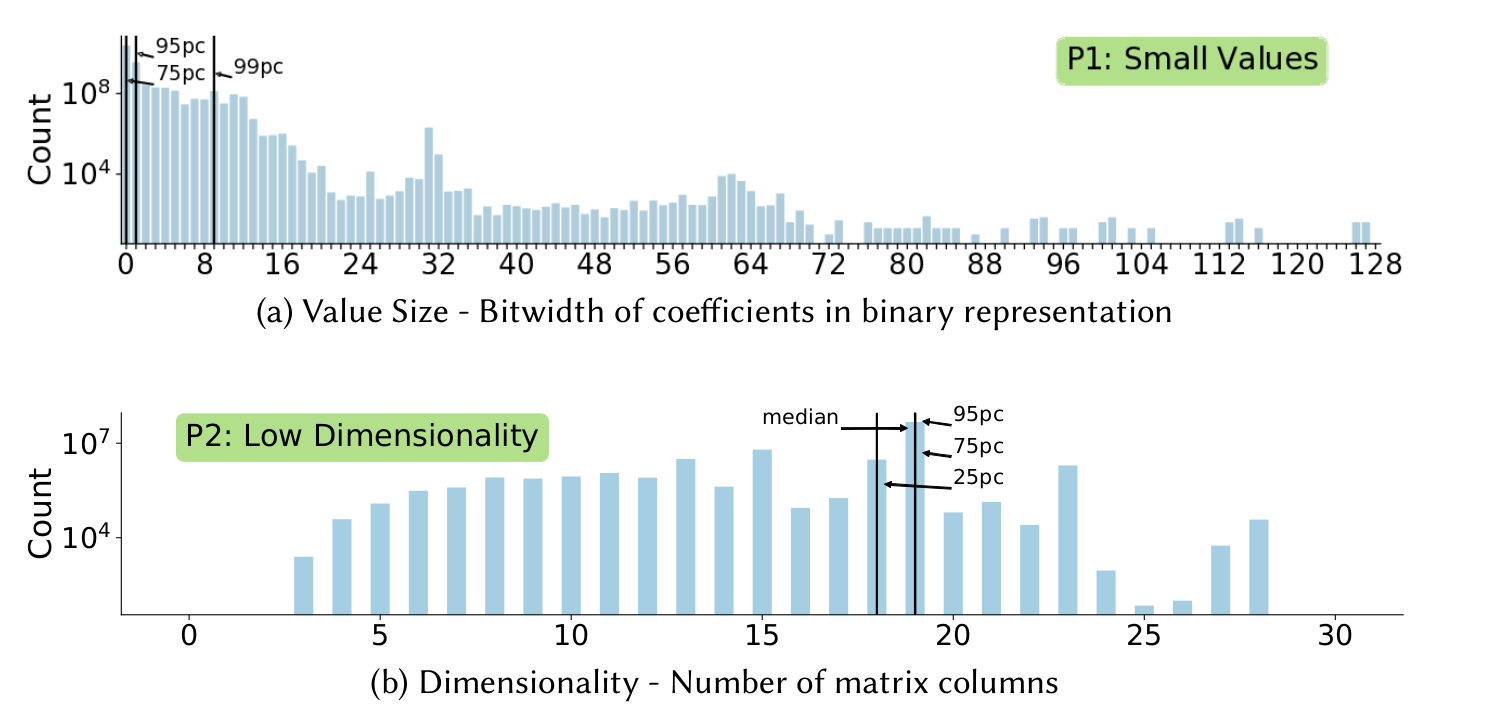
\includegraphics[width=\linewidth]{image/small-val-low-dim.png}
    \caption{TODO.~\cite{FPL1}}
    \label{small-val-low-dim}
\end{figure}


However, in rare and corner cases, there can be larger coefficients up to 127
bits. Practically, the upper bound of coefficient size is unknown, making it
required to have arbitrary precision arithmetic \texttt{LargeInteger} as a
backup. Also, the maximum observed column count is 28 and there is not a certain
maximum column count as well. 

The FPL paper presents a 3-way transprecision implementation for the Presburger
library's simplex solver using the algorithm described in Section \ref{simplex}.
It starts from row-wise vectorized \dtshort{}, and will switch to  element-wise
scalar \dtlong{} or element-wise scalar \texttt{LargeInteger} in case of
overflow, as illustrated in Figure \ref{fig:fpl_arch}. But unfortunately the
MLIR upstream only presents a 2-layer transprecision, consisting of element-wise
scalar operation using \dtlong{} and \texttt{LargeInteger}. The \dtshort{}
version is not merged with the upstream for two reasons: 
\begin{compactlist} 
    \item \dtshort{} vectors require \texttt{AVX-512} ISA extension, but hardware
    support is rare (Section \ref{sec:avx512}). 
    \item Despite the \dtshort{} version is fast, overflow checking overhead is
    65\%~\cite{FPL2}. Using floating points could significantly reduce this
    overhead and potentially be faster (Section \ref{sec:i23}).  
\end{compactlist}


\begin{figure}
    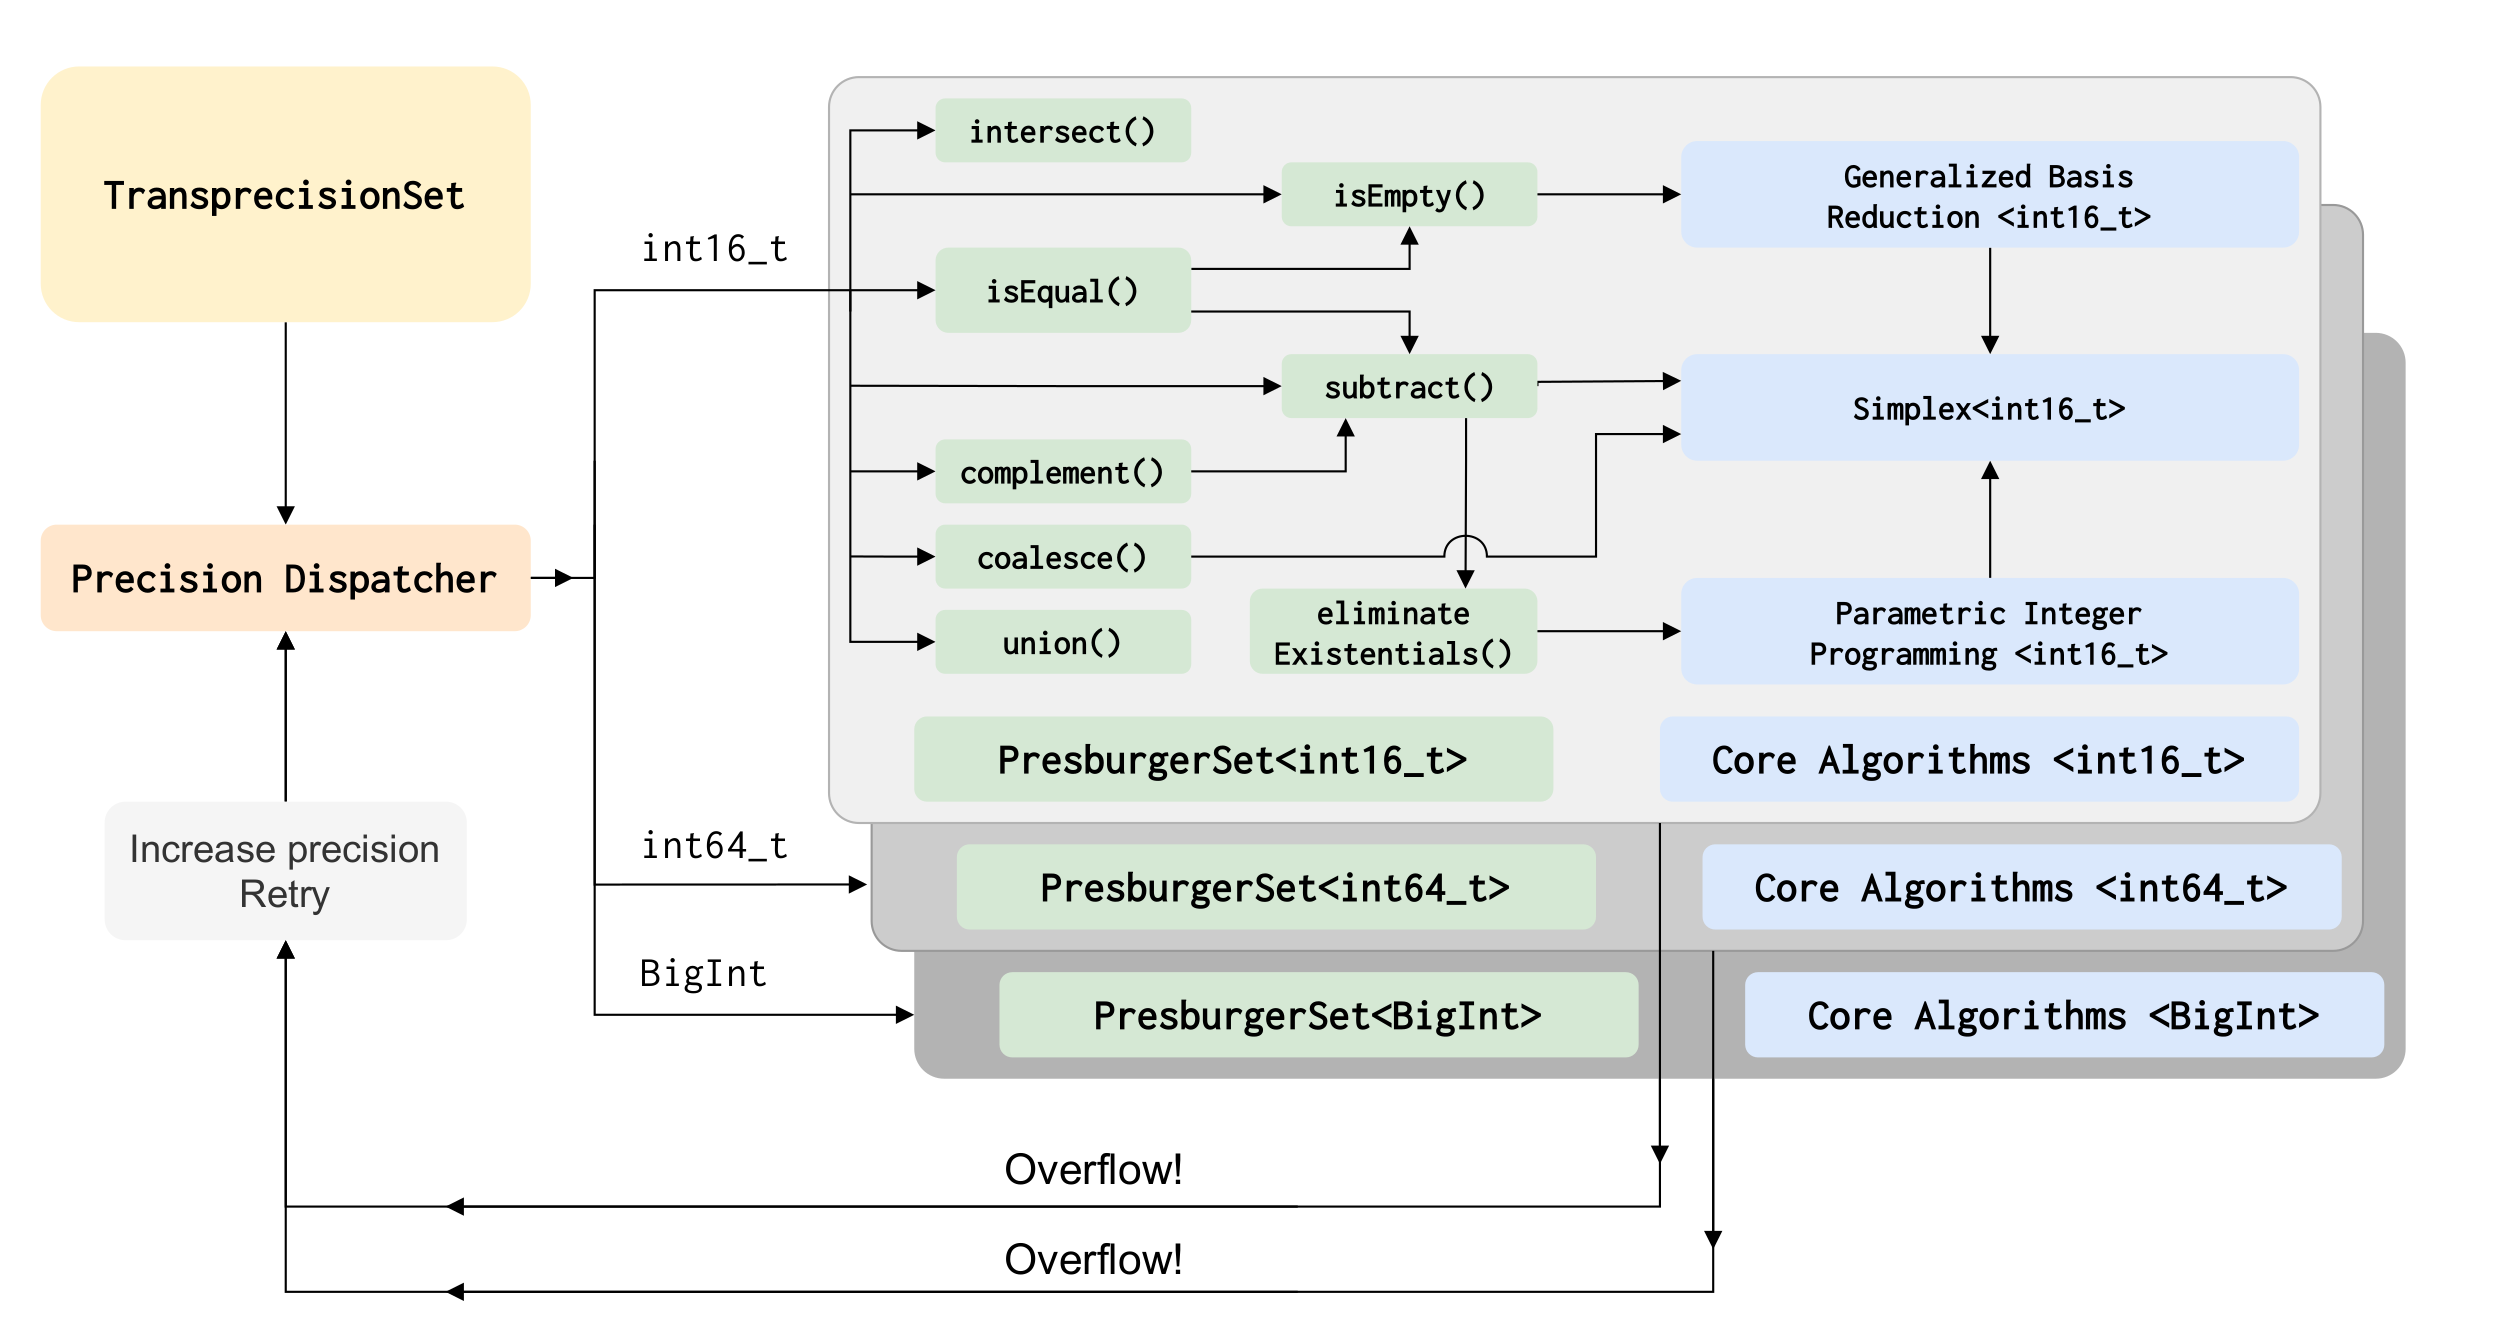
\includegraphics[width=\linewidth]{image/transprecision.png}
    \caption{The The architecture of FPL.}
    \label{fig:fpl_arch}
\end{figure}

\section{Modern CPU micro-architecture}
\label{sec:avx512}

A recent trend in x86-64 architecture’s development is to include \texttt{AVX-512}
instruction set architecture (ISA) extension. \texttt{AVX-512} succeeds \texttt{AVX-2}, the vector
width is increased from \texttt{AVX-2}’s 256 bits to 512 bits. \texttt{AVX-512} also provides new
instructions, for example, \dtshort{} saturated addition.

\subsection{Intel}

Even though its specification was released by Intel in 2013, it had been
unpopular ~\cite{linusHopeAvx512Die}, as it did not bring practical performance
improvements. The primary reason was that it consumed a lot more power than
usual, causing severe overheating. The micro-architecture Skylake from Intel,
and its \texttt{AVX-512} enabled counterpart Skylake-X is a classic example.
Skylake provides 2 256 bits FMA \texttt{AVX-2} execution units
\footnote{Fused-multiply-add (FMA) execution units are a type of floating point
execution units, capable of doing addition, multiplication or both in a single
instruction. See Section \ref{sec:FMA}.} and Intel provides 2 512-bit
\texttt{AVX-512} FMA units by fusing the existing \texttt{AVX-2}  units into a
\texttt{AVX-512} unit, then introduces an additional FMA \texttt{AVX-512}
unit~\cite{SLK-X}. The additional \texttt{AVX-512} unit increases the heat flux
density of the chip, causing server thermal throttling issues. 

Intel attempted to mitigate this problem by introducing the
``\texttt{AVX-offset}'' mode. When a workload involving \texttt{AVX-512}
instructions is encountered, the CPU automatically enters the
\texttt{AVX-offset} mode and reduces its clock frequency \cite{AVX-offset}. This
solution only works in theoretical benchmarks where \texttt{AVX-512}
instructions presents in large bulk, but in practice it is more common to have a
mix of control flow, scalar, \texttt{SSE} and \texttt{AVX-512} instructions. The
clock frequency of executing those non-\texttt{AVX-512} instructions is
decreased together with \texttt{AVX-512} instructions, causing many workloads
could run faster with disabled \texttt{AVX-512} and higher clock
frequency~\cite{Zen4Critique}. 

\hlc[pink]{OptionalTODO: alderlake disabled avx-512 for big.LITTLE}


\subsection{AMD}
AMD recently decides to add support for \texttt{AVX-512} in their latest
micro-architecture Zen4. It has slightly less computing power comparing with
Intel, but much more efficient. Zen4 can be considered as modernized version of
Zen3 or Zen2, where Zen2 and Zen3 supports \texttt{AVX-2}  by providing 2 FADD
units \footnote{Floating-point add units (FADD) can execute addition
instructions only. They may be considered as simplified FMA} and 2 FMA units of
256-bit width \cite{Zen2ChipWiki}. Zen4 ``double-pumps'' these existing circuits
to create a single 512-bit FADD and a single 512-bit FMA, without introducing
any new arithmetic units ~\cite{Zen4Critique}. Zen2 and Zen3 are reputable for
its high performance per watt~\cite{ZenPerfPerWatt}, and Zen4 would be better
with its more advanced lithography~\cite{Zen4Critique}.

Additionally, rebuilding existing software to target \texttt{AVX-512} may bring
slight performance improvement. One benefit of \texttt{AVX-512} is that it
reduces front-end pressure. In the case of the Zen4 micro-architecture, though
the back-end is possible to commit 2 \texttt{AVX-2} FADD and 2 \texttt{AVX-2}
FMA every cycle, the front-end has to dispatch 4 instructions per cycle, which
is quite difficult. The equivalency in \texttt{AVX-512} only takes 2
instructions, this is much more likely to be sustained by the
frontend~\cite{Zen4Critique}.


\section{Floating points}
\label{sec:i23}
\subsection{IEEE 754}
\label{sec:IEEE754}
IEEE 754 is the standard for representing and manipulating floating-point
numbers in modern x86 computers. The standard defines several different formats
for representing floating point numbers, the most common ones are 32-bit single
precision (float) and 64-bit double precision (double). For each format, it
specifies how many bits are used to represent the sign, exponent, and mantissa. 

For float and double, the sign bit is a single bit that indicates whether the
number is positive or negative. As Figure \ref{fig:ieee-f32} shows, there are 8
bits and 11 bits for exponent in float and double respectively, to represent
represents the order of magnitude. The remaining 23 bits in float and 52 bits in
double are mantissae, to store the fractional part of the number. The value of a
floating point number can be computed through this formula: 
\begin{math} (-1)^s * 2^{(e - B)} * (1 + f)\end{math}
where \begin{math}s\end{math} is sign, \begin{math}e\end{math} is exponent, 
\begin{math}f\end{math} is mantissa and \begin{math}B\end{math} is a constant bias
value: \begin{math}127\end{math} for float, \begin{math}1023\end{math} for double. 

Figure \ref{fig:ieee-f32} provides an example of \dtfloat{} by presenting
\texttt{0.15625} in binary form:
\begin{VerbatimCompact}
sign     = 0b0        -> 0
exponent = 0b01111100 -> 0b01111100 - 127 = 124 - 127 = -3
mantissa = 0b01       -> 0b1.01 = 1.25
\end{VerbatimCompact}
Substituting the sign, exponent and mantissa into the formula, we get: \\
\texttt{-1\^{}0 * 2\^{}(-3) * 1.25 = 0.15625}.



\begin{figure}
    \begin{center}
        \captionsetup{justification=centering}
        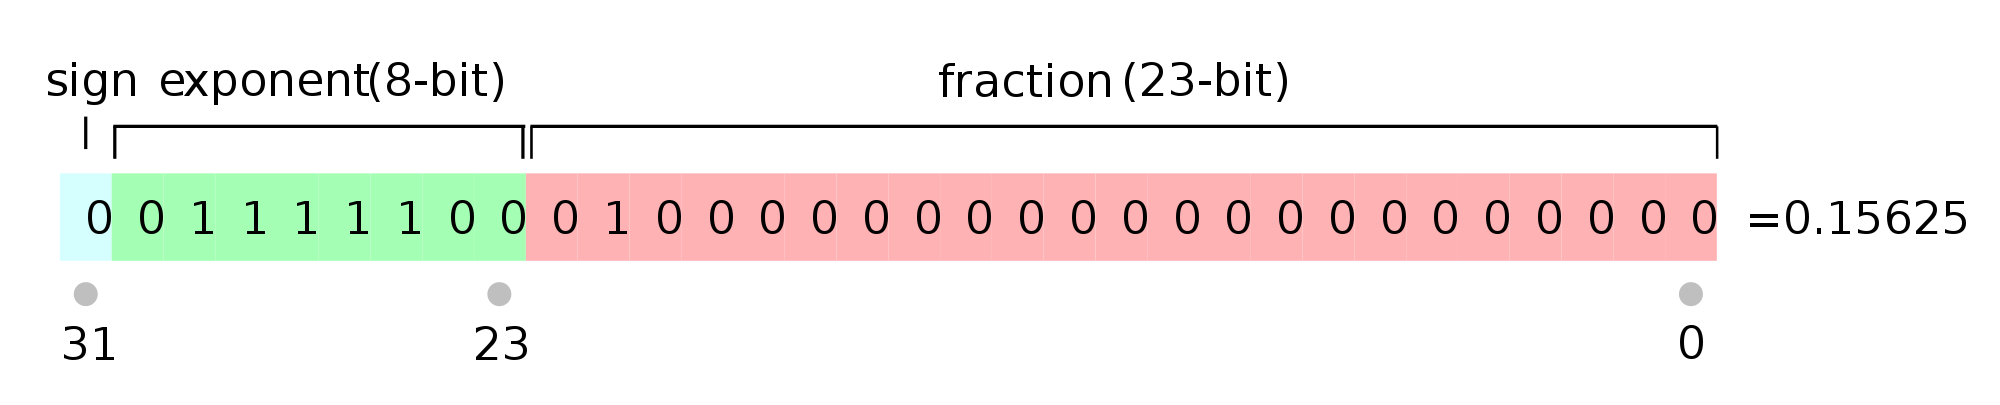
\includegraphics[width=\linewidth]{image/ieee-f32.png}
        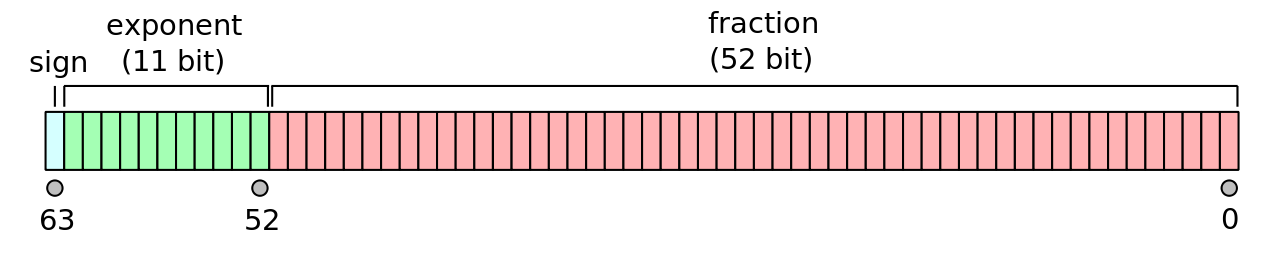
\includegraphics[width=\linewidth]{image/ieee-f64.png}
        \caption{Diagrams of IEEE 754 single (32 bits) and double (64 bits)
        precision floating point~\cite{ieee754-diagram}. In some literature
        ``mantissa'' is referred as ``fraction''.}
        \label{fig:ieee-f32}
    \end{center}
\end{figure}

\subsection{Fused-multiply-add}
\label{sec:FMA}

After doing floating point arithmetic, it is required to normalize the result of
floating-point arithmetic before it can be used further. However, by feeding the
result of a floating-point multiplication (FMUL) directly into the
floating-point addition (FADD) logic without the need for normalization and
rounding in between, a fused multiply-add (FMA) operation is effectively
created: 
\begin{math}Y = (A * B) + C \end{math}, where 
\begin{math}A\end{math},
\begin{math}B\end{math} and
\begin{math}C\end{math} are the operands, 
 \begin{math}Y\end{math} is the result~\cite{CARD}.

FMA saves cycles and reduces accumulation of rounding errors, while at the same
time not adding significant complexity to the circuit. A FMA execution unit is
capable to do FMUL, FADD, and FSUB as well: 
\begin{compactlist} 
\item[] Addition: \begin{math}Y = (A * 1.0) + C \end{math} 
\item[] Multiplication: \begin{math} Y = (A * B) + 0.0 \end{math} 
\item[] Subtraction: \begin{math} Y = (A * -1.0) + C\end{math} 
\end{compactlist} 

This is a useful feature in many numerical computations that involve
simultaneous multiplication and addition operations, such as dot produpreliminaryct and
matrix multiplication. Since the \pivot{} function performs multiplication and
addition between the pivot row, some constant value and each row in the matrix,
the performance of FMA is critical to the overall efficiency of the algorithm. 

\subsection{Representing ``\texttt{int23\_t}'' and ``\texttt{int52\_t}'' using
floating points}
\label{sec:fpe2}

There is a common stereotype that floating-point numbers are unreliable and
likely to be imprecise, and are often illustrated in popular memes (as shown in
Figure \ref{meme}). However, when storing integer values inside floating points, 
floating points can be quite reliable. 

Specifically, given that the mantissa part of a float consists of 23 bits,
inexactness never occur when representing integers less than 23 bits (ignoring
the sign bit). Furthermore, in case of of an integer overflow, floating point
imprecision almost always occurs and a corresponding status registers is set.
The same concept applies to double data types, which have a mantissa consisting
of 52 bits.

This mechanism is reliable, as floating-point inexactness always implies
integer-inexactness. For a integer value with bit width greater than the
mantissa size, floating point rounding is triggered in order to fit most
significant bits of the integer in the mantissa, and then adjust the order of
magnitude in the exponent accordingly. The lower bits of the mantissa are
truncated, therefore causing imprecision. 

In some rare cases, integers longer than the size of mantissa can be represented
in floating points precisely. An examples of such numbers are large powers of 2,
like \texttt{2\^{}30 = 0x40000000}. Its binary representation in \dtfloat{}
is:
\begin{VerbatimCompact}
Sign     = 0
Exponent = 10011011
Mantissa = 0
\end{VerbatimCompact}
Despite being greater than the size of
the mantissa, they are normalized rather then being rounded, and therefore does
not break the mechanism of representing integer in floating-points.

Throughout history, floating point processing units in GPUs have been utilized
for fast integer arithmetic, for example, modular exponentiation
\cite{intfpu-modexp} and RSA algorithms~\cite{intfpu-rsa}, because often the
architecture of GPU prioritizes floating points performance rather than
integers. 
% \hl{TODO: place this paragraph here?}


\begin{figure}
\begin{center}
    
\includegraphics[width=50mm,scale=0.1]{image/0.3004.jpg}
    \caption{A floating point meme: \texttt{0.1 + 0.2 = 0.30000000000000004}}
    \label{meme}
\end{center}
\end{figure}

\section{Google Benchmark}
Google benchmark is a library to measure the performance of a code snippet. It
provides unit-test like interfaces to setup benchmarks around a code snippet
\cite{googlebench}. The given example from https://github.com/google/benchmark
is self-explanatory for its usage: 

\begin{verbatim}
#include <benchmark/benchmark.h>

static void BM_SomeFunction(benchmark::State& state) {
    // Perform setup here
    for (auto _ : state) {
    // This code gets timed
    SomeFunction();
    }
}
// Register the function as a benchmark
BENCHMARK(BM_SomeFunction);
// Run the benchmark
BENCHMARK_MAIN();
\end{verbatim}

The library first starts a timer, repeatedly executes its core loop: \texttt{for
(auto \_ : state) ... } multiple times then pauses the timer. This method
ensures that the results are consistent and minimizes the overhead required for
recording the timing information. 

Executing the benchmarks will not only report both elapsed real time and CPU
time, but also much other useful information to help reduce variance. 
\begin{verbatim}
Running ./build/example
***WARNING*** CPU scaling is enabled, the benchmark real time 
measurements may be noisy and will incur extra overhead.
Run on (32 X 5800.00 MHz CPU s)
CPU Caches:
    L1 Data 32 KiB (x16)
    L1 Instruction 32 KiB (x16)
    L2 Unified 1024 KiB (x16)
    L3 Unified 32768 KiB (x2)
Load Average: 8.10, 5.14, 1.14
----------------------------------------------------------
Benchmark                Time             CPU   Iterations
----------------------------------------------------------
BM_SomeFunction       18.5 ns         18.5 ns     37935734
\end{verbatim}

The warning: ``CPU scaling is enabled, the benchmark real-time measurements may
be noisy and will incur extra overhead.'' is saying that CPU clock frequency is
not consistent. It can be dynamically determined by the governor algorithm,
according on the system's needs. For example, with the \texttt{performance}
governor, the OS locks the CPU to the highest possible clock frequency,
specified at \texttt{/sys/devices/system/cpu/cpu*/cpufreq/scaling\_max\_freq},
while the \texttt{ondemand} governor will push the CPU to the highest frequency
on demand and then gradually reduce the frequency as the idle time increases
\cite{archLinuxFreqScal}.

However, it is also dependent on the manufacture and other hardware constraints.
By default, both Intel (Turbo Boost) and AMD (Precision Boost Overdrive) have
support for raising clock frequency, beyond the control of the governor
\cite{GoogleBenchReduceVariance}. On the other hand, CPUs have self-protecting
thermal throttling mechanisms that reduces its clock frequency and voltage when
it is too hot. 

The benchmark mentioned in this report were performed on a AMD 7950x desktop
computer. The computer system went through the following these setups for
consistent results:
\begin{compactlist}
    \item Set the governor to \texttt{performance}, 
    \item Disable AMD Precision Boost Overdrive (or Intel Turbo Boost), 
    \item Lock clock frequency at a 5 GHz, or any desired fixed value,
    \item Make sure heat dissipation is working properly.
\end{compactlist}



\section{\mca{}}

\mca{}, LLVM Machine Code Analyzer, is a tool to analyze performance of executing
some instructions on a specific CPU micro-architecture, according to scheduling
information provided by LLVM~\cite{llvm-mca}. 

By supplying \mca{} with a piece of assembly code and the target
micro-architecture codename, \mca{} reports various metrics to indicate how fast
the given instructions will execute on the specified micro-architecture. It
first summarizes the instruction per clock (IPC) and throughput of the entire
instruction block, then gives detailed information about each instruction,
including number of uOps, latency, throughput, potential load, store and side
effects. \mca{} also reports resource pressure in terms of arithmetic units and
memory load or store units. When the optional \texttt{-timeline} flag is
prompted, \mca{} illustrates a timeline view of the analyzed code, showing how
instructions progress through the pipeline stages of the target processor. The
timeline helps understand the capability of complicated out-of-order superscalar
architecture. 

An example is provided below. The analysis from \mca{} indicates that a \texttt{znver2}
(Zen2) CPU can repeatedly execute a combination of 
\texttt{vmovaps}\footnote{\texttt{vmovaps} can be either vector float load or 
store instruction, depending on how operands are structured.}
and \texttt{vfmadd213ps}\footnote{\texttt{vfmadd213ps} is the instruction for 
fused-multiply-add.}
instructions every 1.3 cycle. This translates to 2.74 instructions per cycle. 
The output from \mca{} is slightly modified and truncated to fit into 
limited page size. 
% $ cat x.s
% vmovaps (%rdx,%rsi,4),%ymm0
% vmovaps (%rcx,%rax,4),%ymm1
% vfmadd213ps (%r8,%rdi,4),%ymm0,%ymm1
% vmovaps %ymm1,(%r9,%rax,4)

\begin{verbatim}
$ llvm-mca-15 -timeline -mcpu=znver2 ./x.s 
Iterations:        100
Instructions:      400
Total Cycles:      146
Total uOps:        400

Dispatch Width:    4
uOps Per Cycle:    2.74
IPC:               2.74
Block RThroughput: 1.3

Instruction Info:
[1]: #uOps
[2]: Latency
[3]: RThroughput
[4]: MayLoad
[5]: MayStore
[6]: HasSideEffects (U)

[1] [2] [3]  [4] [5] [6] Instructions:
 1   8  0.33  *          vmovaps  (%rdx,%rsi,4), %ymm0
 1   8  0.33  *          vmovaps  (%rcx,%rax,4), %ymm1
 1   12 0.50  *          vfmadd213ps  (%r8,%rdi,4), %ymm0, %ymm1
 1   1  0.33      *      vmovaps  %ymm1, (%r9,%rax,4)

Resources:
[0]   - Zn2AGU0
[1]   - Zn2AGU1
[2]   - Zn2AGU2
...
[8]   - Zn2FPU0
[9]   - Zn2FPU1
[10]  - Zn2FPU2
[11]  - Zn2FPU3
[12]  - Zn2Multiplier

Resource pressure per iteration:
[0]  [1]  [2]  [3] [4] [5] [6] [7] [8]  [9] [10] [11] [12]   
1.33 1.33 1.34  -   -   -   -   -  0.50  -   -   0.50  -     

Resource pressure by instruction:
[0]  [1]  [2]  ... [8]  [11] Instructions:
0.01 0.38 0.61 ...  -    -   vmovaps  (%rdx,%rsi,4), %ymm0
0.23 0.68 0.09 ...  -    -   vmovaps  (%rcx,%rax,4), %ymm1
0.27 0.24 0.49 ... 0.50 0.50 vfmadd213ps  (%r8,%rdi,4), %ymm0, %ymm1
0.82 0.03 0.15 ...  -    -   vmovaps  %ymm1, (%r9,%rax,4)

Timeline view:
                0123456789      
Index 0123456789          012345

[0,0] DeeeeeeeeER    .    .    . vmovaps  (%rdx,%rsi,4), %ymm0
[0,1] DeeeeeeeeER    .    .    . vmovaps  (%rcx,%rax,4), %ymm1
[0,2] D=eeeeeeeeeeeeER    .    . vfmadd213ps  (%r8,%rdi,4), %ymm0, %ymm1
[0,3] D=============eER   .    . vmovaps  %ymm1, (%r9,%rax,4)
[1,0] .DeeeeeeeeE-----R   .    . vmovaps  (%rdx,%rsi,4), %ymm0
[1,1] .DeeeeeeeeE-----R   .    . vmovaps  (%rcx,%rax,4), %ymm1
[1,2] .D=eeeeeeeeeeeeER   .    . vfmadd213ps  (%r8,%rdi,4), %ymm0, %ymm1
[1,3] .D=============eER  .    . vmovaps  %ymm1, (%r9,%rax,4)
[2,0] . DeeeeeeeeE-----R  .    . vmovaps  (%rdx,%rsi,4), %ymm0
[2,1] . DeeeeeeeeE-----R  .    . vmovaps  (%rcx,%rax,4), %ymm1
...

\end{verbatim}


% [2,2] . D=eeeeeeeeeeeeER  .    . vfmadd213ps  (%r8,%rdi,4), %ymm0, %ymm1
% [2,3] . D=============eER .    . vmovaps  %ymm1, (%r9,%rax,4)
% [3,0] .  DeeeeeeeeE-----R .    . vmovaps  (%rdx,%rsi,4), %ymm0
% [3,1] .  DeeeeeeeeE-----R .    . vmovaps  (%rcx,%rax,4), %ymm1
% [3,2] .  D=eeeeeeeeeeeeER .    . vfmadd213ps  (%r8,%rdi,4), %ymm0, %ymm1
% [3,3] .  D=============eER.    . vmovaps  %ymm1, (%r9,%rax,4)
% [4,0] .   DeeeeeeeeE-----R.    . vmovaps  (%rdx,%rsi,4), %ymm0
% [4,1] .   DeeeeeeeeE-----R.    . vmovaps  (%rcx,%rax,4), %ymm1
% [4,2] .   D=eeeeeeeeeeeeER.    . vfmadd213ps  (%r8,%rdi,4), %ymm0, %ymm1
% [4,3] .   D=============eER    . vmovaps  %ymm1, (%r9,%rax,4)
% [5,0] .    DeeeeeeeeE-----R    . vmovaps  (%rdx,%rsi,4), %ymm0
% [5,1] .    DeeeeeeeeE-----R    . vmovaps  (%rcx,%rax,4), %ymm1
% [5,2] .    D=eeeeeeeeeeeeER    . vfmadd213ps  (%r8,%rdi,4), %ymm0, %ymm1
% [5,3] .    D=============eER   . vmovaps  %ymm1, (%r9,%rax,4)
% [6,0] .    .DeeeeeeeeE-----R   . vmovaps  (%rdx,%rsi,4), %ymm0
% [6,1] .    .DeeeeeeeeE-----R   . vmovaps  (%rcx,%rax,4), %ymm1
% [6,2] .    .D=eeeeeeeeeeeeER   . vfmadd213ps  (%r8,%rdi,4), %ymm0, %ymm1
% [6,3] .    .D=============eER  . vmovaps  %ymm1, (%r9,%rax,4)
% [7,0] .    . DeeeeeeeeE-----R  . vmovaps  (%rdx,%rsi,4), %ymm0
% [7,1] .    . DeeeeeeeeE-----R  . vmovaps  (%rcx,%rax,4), %ymm1
% [7,2] .    . D=eeeeeeeeeeeeER  . vfmadd213ps  (%r8,%rdi,4), %ymm0, %ymm1
% [7,3] .    . D=============eER . vmovaps  %ymm1, (%r9,%rax,4)
% [8,0] .    .  DeeeeeeeeE-----R . vmovaps  (%rdx,%rsi,4), %ymm0
% [8,1] .    .  DeeeeeeeeE-----R . vmovaps  (%rcx,%rax,4), %ymm1
% [8,2] .    .  D=eeeeeeeeeeeeER . vfmadd213ps  (%r8,%rdi,4), %ymm0, %ymm1
% [8,3] .    .  D=============eER. vmovaps  %ymm1, (%r9,%rax,4)
% [9,0] .    .   DeeeeeeeeE-----R. vmovaps  (%rdx,%rsi,4), %ymm0
% [9,1] .    .   DeeeeeeeeE-----R. vmovaps  (%rcx,%rax,4), %ymm1
% [9,2] .    .   D=eeeeeeeeeeeeER. vfmadd213ps  (%r8,%rdi,4), %ymm0, %ymm1
% [9,3] .    .   D=============eER vmovaps  %ymm1, (%r9,%rax,4)


% Average Wait times (based on the timeline view):
% [0]: Executions
% [1]: Average time spent waiting in a scheduler's queue
% [2]: Average time spent waiting in a scheduler's queue while ready
% [3]: Average time elapsed from WB until retire stage

%       [0]    [1]    [2]    [3]
% 0.     10    1.0    1.0    4.5       vmovaps	(%rdx,%rsi,4), %ymm0
% 1.     10    1.0    1.0    4.5       vmovaps	(%rcx,%rax,4), %ymm1
% 2.     10    2.0    0.0    0.0       vfmadd213ps	(%r8,%rdi,4), %ymm0, %ymm1
% 3.     10    14.0   0.0    0.0       vmovaps	%ymm1, (%r9,%rax,4)
%        10    4.5    0.5    2.3       <total>

% \end{verbatim}

However, when evaluating the identical assembly code on a more advanced
micro-architecture \texttt{znver3} (Zen3), \mca{} reveals reduction in IPC and
throughput. This appears to be contradictory with both theoretical expectations
and actual benchmarks. After submitting an
\href{https://github.com/llvm/llvm-project/issues/59325}{issue}
\cite{mca-issue}, llvm maintainers explained that llvm's scheduling information
are hand-crafted using \exegesis{}, a micro-benchmark tool. The issue was
subsequently resolved after rerunning \exegesis{} and confirming that
\texttt{znver3} indeed has higher throughput as expected. 

\hl{TODO: should I
write a paragraph to emphacise that \mca{} is unreliable?}

\chapter{Experiments with Toy Example}
\label{sec:Toy}

The \pivot{} function does multiply and add for each row in the matrix,
therefore the performance of FMA a simple vector toy can be an effective
indicator. This chapter reports performance analysis on simple toy examples that
do vector add or vector FMA with various setups, including: 

\begin{enumerate} 
    \item Vectorization method 
        \begin{compactlist} 
            \item Clang's automatic vectorization from scalar source code
            \item Clang builtin vector datatype with occasional AVX intrinsics 
        \end{compactlist}
    \item Matrix data structure 
        \begin{compactlist} 
            \item Nested list
            \item Flat list
        \end{compactlist}
    \item Element data width
        \begin{compactlist} 
            \item 16 bits: \dtshort{}
            \item 32 bits: \dtint{}, \dtfloat{}
            \item 64 bits: \dtlong{}, \dtdouble{}
        \end{compactlist}
    \item Element data type 
        \begin{compactlist} 
            \item Integer
            \item Floating point
        \end{compactlist}
\end{enumerate}

\section{Vectorization method}
\label{sec:vectorization-method}
\subsection{Clang's automatic vectorization}
Clang is capable of generating vectorized instructions from scalar source code,
using the flags \texttt{-O3 -march=native} on a platform with vector ISA
enabled. Starting with an example (Listing \ref{vec-add-float-auto}), the simple
\texttt{vec\_add} function adds every element from two arrays and saves it to
the third. 

\begin{table}[ht]\captionsetup{name=Listing}
\captionsetup{justification=centering}
\begin{tabular}{>{\raggedright\arraybackslash}p{14cm}}
    Source code\\
    \midrule
    \begin{VerbatimCompact}
#define size 128
void vec_add(float* src1_ptr, float* src2_ptr, float* dst_ptr) {
    for (uint32_t i = 0; i < size; i += 1 ){
        dst_ptr[i] = src1_ptr[i] + src2_ptr[i];
    }
}
    \end{VerbatimCompact}
    \\

    Assembly snippet of the hot loop, vectorization on\\
    \midrule
    \begin{VerbatimCompact}
1458: c4 c1 7c 58 84 87 20   vaddps -0x1e0(%r15,%rax,4),%zmm0,%zmm0
145f: fe ff ff
1462: c4 c1 74 58 8c 87 40   vaddps -0x1a0(%r15,%rax,4),%zmm1,%zmm1
1469: fe ff ff
    \end{VerbatimCompact}
    \\
    Assembly snippet of the hot loop, vectorization off\\
    \midrule
    \begin{VerbatimCompact}
120d: d8 44 82 04    fadds  0x4(%rdx,%rax,4)
1211: d9 5c 81 04    fstps  0x4(%rcx,%rax,4)
1215: d9 44 86 08    flds   0x8(%rsi,%rax,4)
    \end{VerbatimCompact}
\end{tabular}
\caption{The vectorized and scalar binary are derived by compiling with flags
\texttt{-O3 -march=native} and \texttt{-O3 -march=native -mno-avx -mno-sse}
respectively, on a Zen4 computer with \texttt{clang-17}.}
\label{vec-add-float-auto}
\end{table}
% \hl{TODO: these hex code are actually incorrect, I assume this does not really matter?}

After compiling on a \texttt{AVX-512} enabled computer and disassembling the
binary, it is observed that clang automatically packs 16 \dtfloat{} (512 bits)
as a operand of the \texttt{vaddps} instruction. 

Alternatively, vectorization could be disabled by adding the \texttt{-mno-avx
-mno-sse} flags on top of \texttt{-O3 -march=native}. These two sets of flags
guarantee that the binary are going to be equally optimized, with the only
difference been whether vector instructions are generated or not. In this case,
scalar instructions \texttt{fadds}, \texttt{fstps} and \texttt{flds} are
selected.


\subsection{Clang's vector datatype and AVX intrinsics}

Another approach is to write source code with vectorization in mind in the first
place. Clang provides extension that allows programmers to declare a new type
that represents a vector of elements of the same data type. The syntax is 
\begin{VerbatimCompact}[commandchars=\\\{\}]
typedef \textit{ty} \textit{vec_ty} __attribute__((ext_vector_type(\textit{vec_width}))), 
\end{VerbatimCompact}
where \textit{\texttt{vec\char`_ty}} is the name of vector type being defined,
\textit{\texttt{vec\char`_width}} is its size and \textit{\texttt{ty}} is the
type of the elements in the vector. For example, 
\begin{VerbatimCompact}[commandchars=\\\{\}]
typedef int16_t int16x32 __attribute__((ext_vector_type(32)))
\end{VerbatimCompact}
defines a 512-bit vector type of \texttt{int16x32}, consisting of 32
\texttt{int16\char`_t} and fits inside an \texttt{AVX-512} ZMM register. 

After defining a vector datatype, a vector variable can be created by casting
from a pointer of the target array. Then arithmetic operators can be applied
between the vectors to performed element-wise operations. The previous
\texttt{vec\_add} example can be rewritten as the code snippet shown in Listing
\ref{vec-add-float-vecty}:

\begin{table}[ht]\captionsetup{name=Listing}
\captionsetup{justification=centering}
\begin{tabular}{>{\raggedright\arraybackslash}p{14cm}}
    Source code\\
    \midrule
    \begin{VerbatimCompact}
#define size 128
#define FloatZmmSize 16
typedef float floatZmm __attribute__((ext_vector_type(FloatZmmSize)));
void vec_add(float* src1_ptr, float* src2_ptr, float* dst_ptr) {
    for (uint32_t i = 0; i < size; i += FloatZmmSize){
        floatZmm src1Vec = *(floatZmm *)(src1_ptr + i);
        floatZmm src2Vec = *(floatZmm *)(src2_ptr + i);
        *(floatZmm *)(dst_ptr + i) = src1Vec + src2Vec;
    }
}
\end{VerbatimCompact}
\end{tabular}
\caption{Comparing to Listing \ref{vec-add-float-auto}, it is slightly more
complicated to code with vector types.}
\label{vec-add-float-vecty}
\end{table}
\subsection{Evaluation}

\label{sec:vectorization-method-eval}
When comparing the performance of code written with and without the vector type
and examining their assembly, it has been discovered that the the automatic
vectorization feature in clang can be unpredictable and may lead to undesired
behaviors. It operates as a black box and may take a lot of effort to understand
its mechanisms. One of the issues is that clang may select a suboptimal vector
width.

Consider the \texttt{vec\_fma} function in Listing \ref{table:vec-fma-float}, a
slightly more complicated version of the previous \texttt{vec\_add} example,
where there are 3 input matrices and the element-wise operation is changed from
addition to FMA. The disassembly reveals that clang decides to use FMA vector
instructions of 128-bit width, but when vector size is constrained to a bigger
width by defining a vector type, more optimal binary can be generated. Benchmark
(Figure \ref{plot_vectorization_method}) shows that the vector type version is 6
times and 11 times faster than the automatic vectorization and vectorization
disabled version respectively.

\begin{table}[H]\captionsetup{name=Listing}
\captionsetup{justification=centering}
\begin{tabular}{>{\raggedright\arraybackslash}p{14cm}}
    Source code for clang automatic vectorization\\
    \midrule
    \begin{VerbatimCompact}
void vec_fma(matrix<float> & mat_src1, matrix<float> & mat_src2, 
             matrix<float> & mat_src3, matrix<float> & mat_dst) {
    for (int i = 0; i < row; i += 1) {
        for (int j = 0; j < col; j += 1) {
            float src1 = mat_src1.get(i,j);
            float src2 = mat_src2.get(i,j);
            float src3 = mat_src3.get(i,j);
            mat_dst.set(i,j,  (src1 * src2) + src3);
        }
    }
}
    \end{VerbatimCompact}
    \\
    % \toprule
    Assembly snippet of the hot loop\\
    \midrule
    \begin{VerbatimCompact}
80e4: c5 fa 10 04 b2     vmovss (%rdx,%rsi,4),%xmm0
80f1: c5 fa 10 0c 81     vmovss (%rcx,%rax,4),%xmm1
80fe: c4 c2 79 a9 0c b8  vfmadd213ss (%r8,%rdi,4),%xmm0,%xmm1
810c: c4 c1 7a 11 0c 81  vmovss %xmm1,(%r9,%rax,4)
    \end{VerbatimCompact}
    \\
\\
% \end{tabular}
% \caption{}
% \label{table:vec-fma-float-auto}
% \end{table}

% \begin{table}[H]\captionsetup{name=Listing}
% \begin{tabular}{>{\raggedright\arraybackslash}p{14cm}}
    Source code written with clang's vector type\\
    \midrule
    \begin{VerbatimCompact}
#define FloatZmmSize 16
typedef float floatZmm __attribute__((ext_vector_type(FloatZmmSize)));
void vec_fma(matrix<float> & mat_src1, matrix<float> & mat_src2, 
             matrix<float> & mat_src3, matrix<float> & mat_dst) {
    float * src1_ptr = (float *) mat_src1.getItemPointer(0,0);
    float * src2_ptr = (float *) mat_src2.getItemPointer(0,0);
    float * src3_ptr = (float *) mat_src3.getItemPointer(0,0);
    float * dst_ptr  = (float *) mat_dst.getItemPointer(0,0);
    for (uint32_t i = 0; i < row * col; i += FloatZmmSize){
        floatZmm src1Vec = *(floatZmm *)(src1_ptr + i);
        floatZmm src2Vec = *(floatZmm *)(src2_ptr + i);
        floatZmm src3Vec = *(floatZmm *)(src3_ptr + i);
        *(floatZmm *)(dst_ptr + i) = src1Vec * src2Vec + src3Vec;
    }
}
    \end{VerbatimCompact}
    \\
    % \toprule
    Assembly snippet of the hot loop\\
    \midrule
    \begin{VerbatimCompact}
82c0: 62 b1 7c 48 10 04 80   vmovups (%rax,%r8,4),%zmm0
82c7: 62 b1 7c 48 10 0c 81   vmovups (%rcx,%r8,4),%zmm1
82ce: 62 b2 7d 48 a8 0c 86   vfmadd213ps (%rsi,%r8,4),%zmm0,%zmm1
82d5: 62 b1 7c 48 11 0c 87   vmovups %zmm1,(%rdi,%r8,4)
    \end{VerbatimCompact}
    \\
\end{tabular}
\caption{The key distinction between two vectorization approaches is the
register types. \texttt{XMM} and \texttt{ZMM} are 128-bit and 512-bit
registers respectively.}
\label{table:vec-fma-float}
\end{table}


In some cases clang could be even worse, it may fail to recognize vectorization
patterns from element-wise loop operations, leading to more reduction in
performance. In the \texttt{vec\_fma} example, by changing the type signature
from \dtfloat{} to \texttt{int}, clang decides to dispatch scalar instructions
for addition (\texttt{add}) and multiplication (\texttt{imul}) completely
(Listing \ref{vec-fma-int}). Their vectorized equivalency \texttt{vpaddd} and
\texttt{vpmulld} is 15 times more performant (Figure
\ref{plot_vectorization_method}).

\begin{figure}[H]\captionsetup{name=Figure}
    \captionsetup{justification=centering}
    \begin{center}
    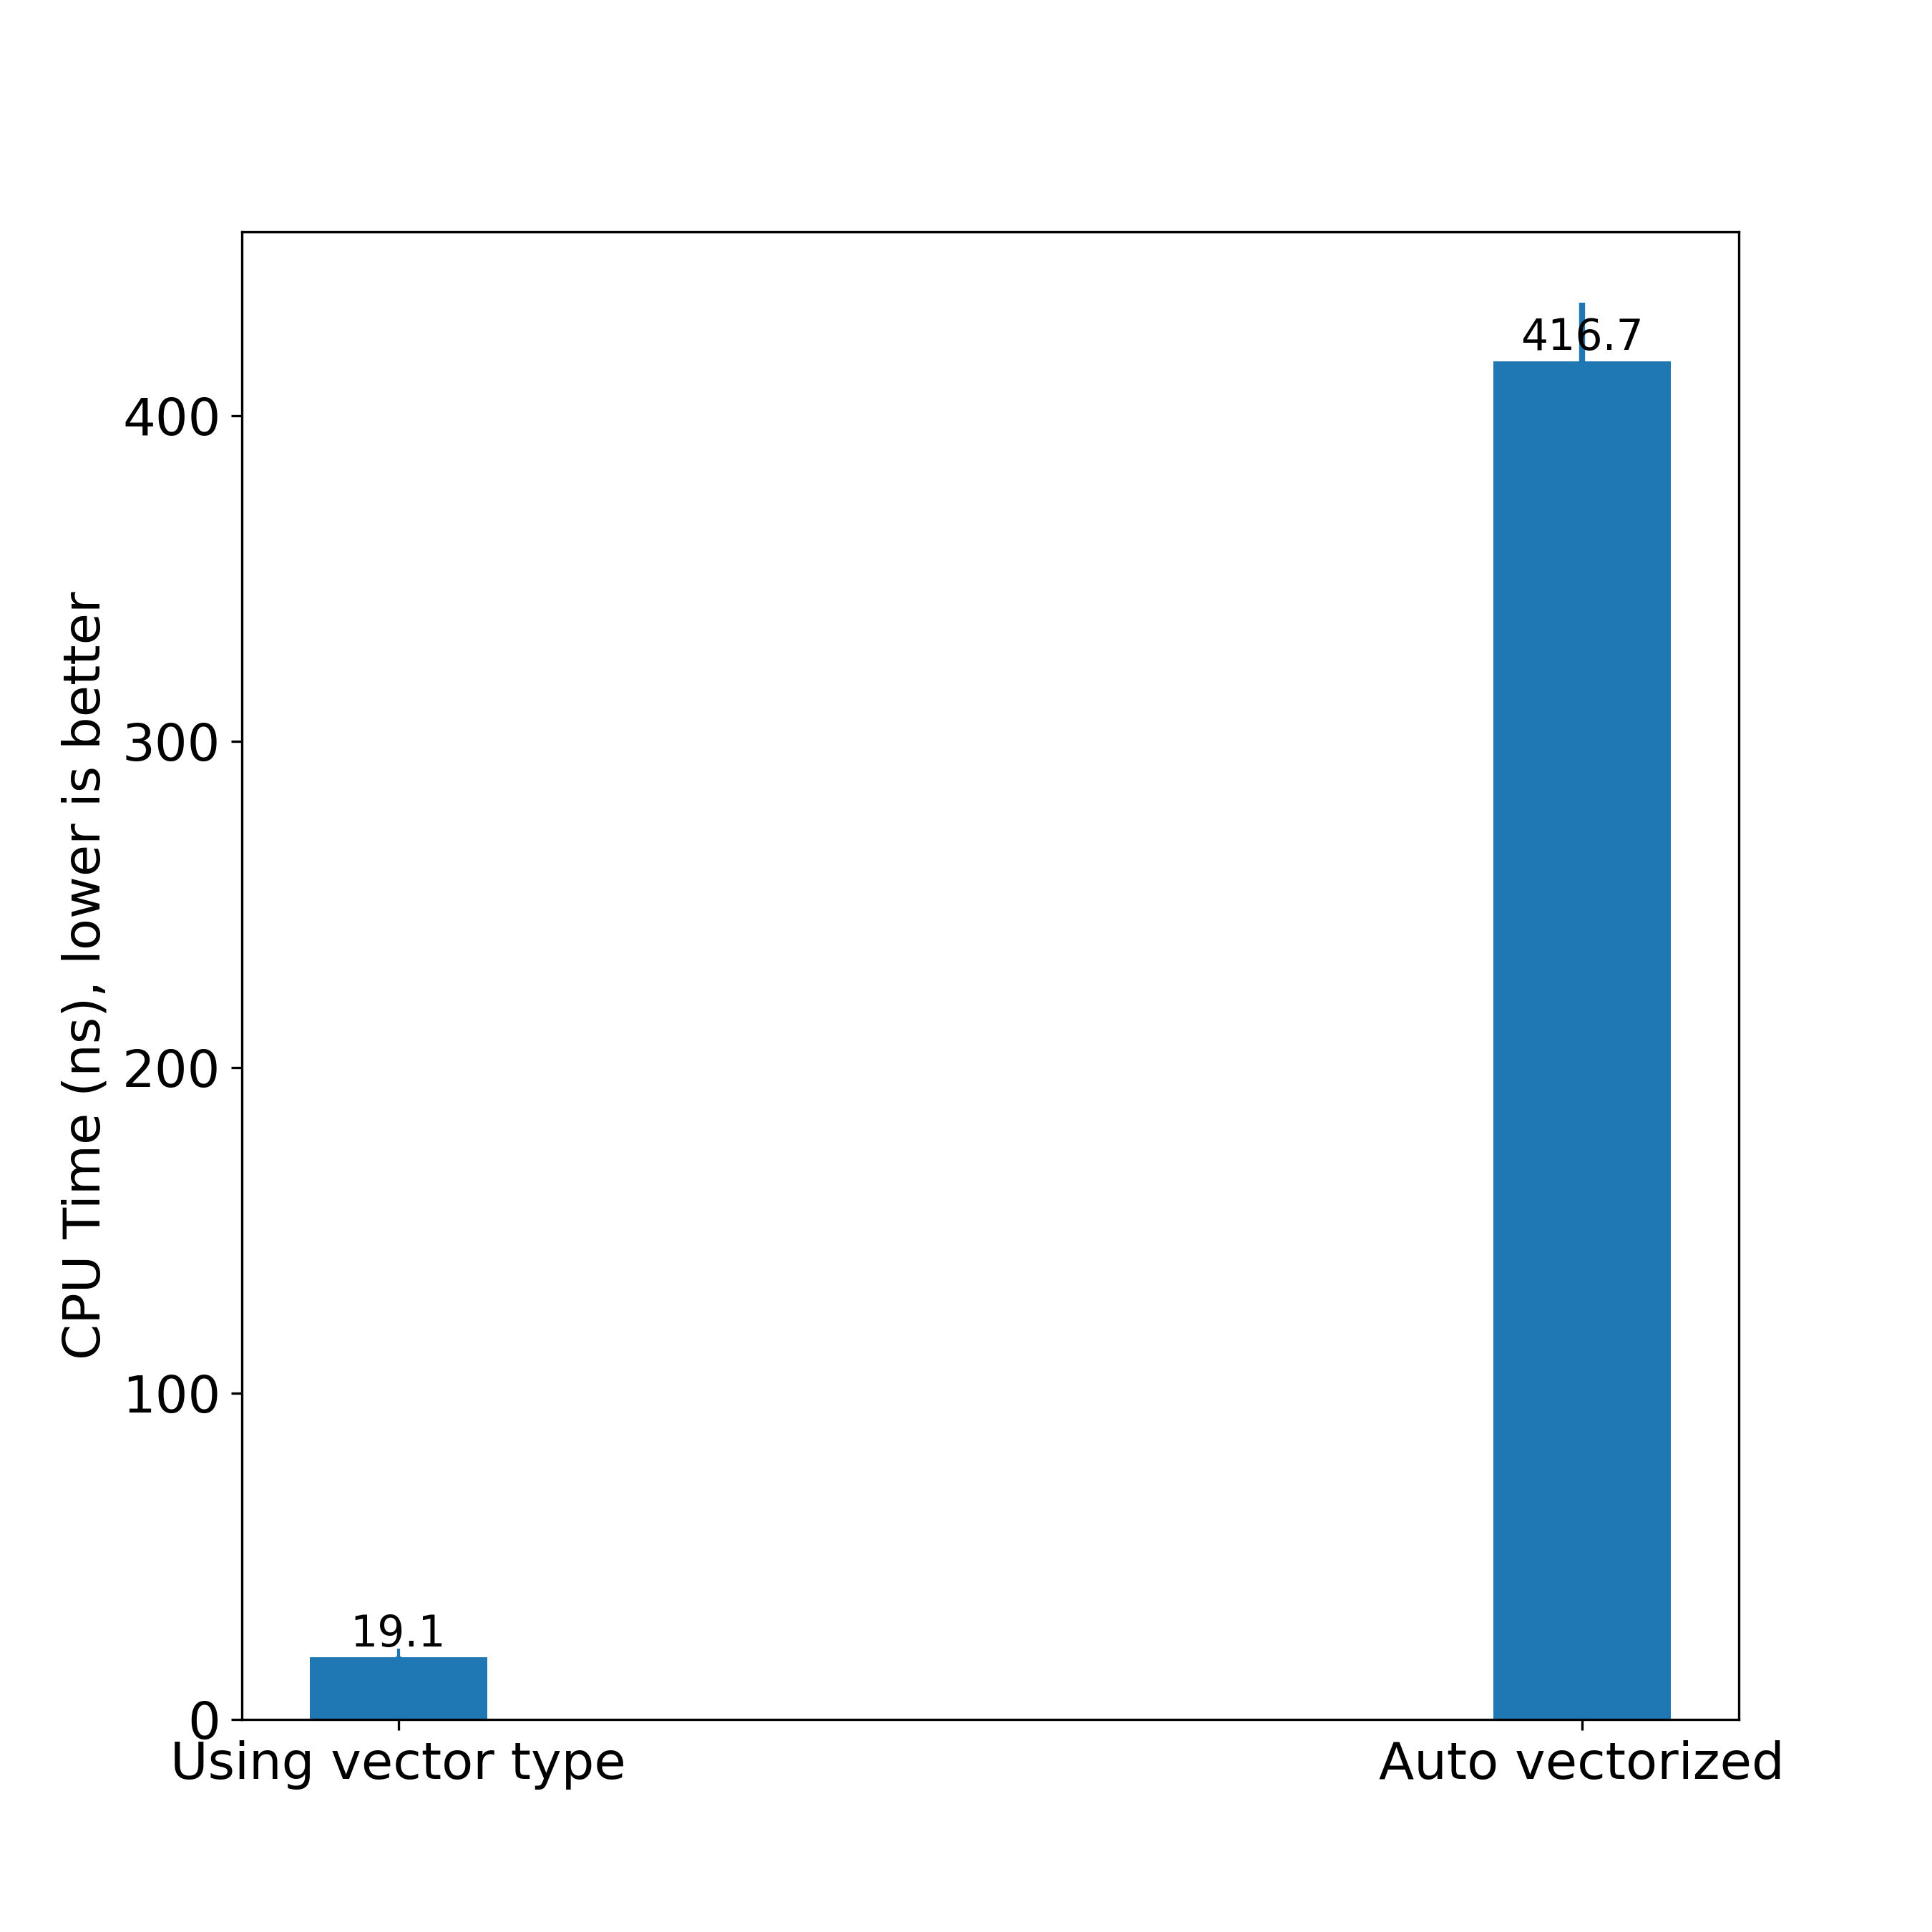
\includegraphics[width=\linewidth]{image/plot_vectorization_method.png}
    \end{center}
    \caption{Source code written with vector type are an order-of-magnitude
    faster than their automatically vectorized or scalar counterpart. Also,
    \dtfloat{} is always faster than \dtint{}, because it benefits from
    fused-multiply-add. }
    \label{plot_vectorization_method}
\end{figure}

    \begin{table}[H]\captionsetup{name=Listing}
\captionsetup{justification=centering}
\begin{tabular}{>{\raggedright\arraybackslash}p{14cm}}
    Source code for clang automatic vectorization\\
    \midrule
    \begin{VerbatimCompact}
void vec_fma(matrix<int> & mat_src1, matrix<int> & mat_src2, 
             matrix<int> & mat_src3, matrix<int> & mat_dst) {
    for (int i = 0; i < row; i += 1) {
        for (int j = 0; j < col; j += 1) {
            int src1 = mat_src1.get(i,j);
            int src2 = mat_src2.get(i,j);
            int src3 = mat_src3.get(i,j);
            mat_dst.set(i,j,  (src1 * src2) + src3);
        }
    }
}
    \end{VerbatimCompact}
    \\
    % \toprule
    Assembly snippet of the hot loop\\
    \midrule
    \begin{VerbatimCompact}
88b0: 44 8b 69 1c  mov    0x1c(%rcx),%r13d
88b4: 44 8b 62 1c  mov    0x1c(%rdx),%r12d
88b8: 45 0f af ee  imul   %r14d,%r13d
88bc: 45 0f af e6  imul   %r14d,%r12d
88c0: 45 01 fd     add    %r15d,%r13d
88c3: 45 01 fc     add    %r15d,%r12d
    \end{VerbatimCompact}
    \\
% \end{tabular}
% \caption{}
% \label{vec-fma-int-auto}
% \end{table}

% \begin{table}[H]\captionsetup{name=Listing}
% \begin{tabular}{>{\raggedright\arraybackslash}p{14cm}}
\\
    Source code written with clang’s vector type\\
    \midrule
    \begin{VerbatimCompact}
#define IntZmmSize 16
typedef int intZmm __attribute__((ext_vector_type(IntZmmSize)));
void vec_fma(matrix<int> & mat_src1, matrix<int> & mat_src2, 
             matrix<int> & mat_src3, matrix<int> & mat_dst) {
    int * src1_ptr = (int *) mat_src1.getItemPointer(0,0);
    int * src2_ptr = (int *) mat_src2.getItemPointer(0,0);
    int * src3_ptr = (int *) mat_src3.getItemPointer(0,0);
    int * dst_ptr  = (int *) mat_dst.getItemPointer(0,0);
    for (uint32_t i = 0; i < row * col; i += IntZmmSize){
        intZmm src1Vec = *(intZmm *)(src1_ptr + i);
        intZmm src2Vec = *(intZmm *)(src2_ptr + i);
        intZmm src3Vec = *(intZmm *)(src3_ptr + i);
        *(intZmm *)(dst_ptr + i) = src1Vec * src2Vec + src3Vec;
    }
}
    \end{VerbatimCompact}
    \\
    % \toprule
    Assembly snippet of the hot loop\\
    \midrule
    \begin{VerbatimCompact}
8880: 62 b1 fe 48 6f 04 81  vmovdqu64 (%rcx,%r8,4),%zmm0
8887: 62 b2 7d 48 40 04 80  vpmulld (%rax,%r8,4),%zmm0,%zmm0
888e: 62 b1 7d 48 fe 04 86  vpaddd (%rsi,%r8,4),%zmm0,%zmm0
8895: 62 b1 fe 48 7f 04 87  vmovdqu64 %zmm0,(%rdi,%r8,4)
    \end{VerbatimCompact}
    \\
\end{tabular}
\caption{Clang fails to vectorize the loop that iterates through
every element, but writing vector type guarantees vectorization. }
\label{vec-fma-int}
\end{table}





\section{Matrix data structure}
\label{sec:mat-structure}
The most intuitive data structure of a matrix is a list of lists, where each
list represents a row and a list of rows is a matrix. In C++ this can be
represented using \texttt{std::vector<std::vector<T>>}, where \texttt{T} could
be \dtfloat{}, \dtdouble{}, \dtint{}, etc. The std::vector
class provides an intuitive interface for accessing and modifying elements,
making it easy to write code with. 

One potential drawback of nested \texttt{std::vector} is that it requires two
indexing operations to access an element. An alternative implementation is to
“flatten” a matrix into a single \texttt{std::vector}, by simply concatenating
one row after another. To access a specific element, an index can be computed
manually using the given row and column: \texttt{column\_count * row + column}.
This reduces half of the memory indexing operation at the cost of additional
arithmetic. The differences between the two patterns are illustrated by a
example provided in Table \ref{table:nested-flat}. 

\begin{table}[ht]
\captionsetup{justification=centering}
\begin{tabular}{%
    >{\raggedright\arraybackslash}p{2cm}%
    >{\raggedright\arraybackslash}p{6.5cm}%
    >{\raggedright\arraybackslash}p{4.5cm}}
    
    \toprule
    & Nested & Flat\\

    \midrule
    
    Type
    &
    \begin{VerbatimCompact}
std::vector<
    std::vector<int32_t>>
    \end{VerbatimCompact}
    &
    \begin{VerbatimCompact}
std::vector<int32_t>
    \end{VerbatimCompact}
    \\

Structure in Memory
    &
    \begin{VerbatimCompact}
vector of 4 = {
    vector of 4 = {0, 0, 0, 0}, 
    vector of 4 = {0, 0, 0, 0}, 
    vector of 4 = {0, 0, 0, 1}, 
    vector of 4 = {0, 0, 0, 0}
}
    \end{VerbatimCompact}
    &
    \begin{VerbatimCompact}
vector of 16 = {
    0, 0, 0, 0, 
    0, 0, 0, 0,
    0, 0, 0, 1, 
    0, 0, 0, 0
}
    \end{VerbatimCompact}
    \\

    Accessing row 2, column 3
    &
    Index row first: \texttt{std::vector<int32\char`_t>[2]} \linebreak
    then index column: 
        \texttt{std::vector<int32\char`_t>[2][3]}
    & 
    Compute \texttt{i = 
    \linebreak col\char`_count * row + col \linebreak = 4 * 2 + 3 =
    11}, \linebreak then index once: \texttt{std::vector<int32\char`_t>[11]}  \\

    \bottomrule

\end{tabular}
\caption{This is an example of a 4 by 4 matrix, to highlight the differences
between the two matrix data structures: nested list and flat list. }
\label{table:nested-flat}
\end{table}

Empirically indexing costs more time than integer multiplication and addition,
thereby improving performance. Both the toy example and the \pivot{} function
perform sequential load-compute-store operations on each row and each column,
allowing the index of the next element to be computed by simply adding the step
size or column size, further reducing memory overhead. In fact, the \pivot{}
function can be optimized to only compute index once (See Section
\ref{sec:optmz-get-index}) by placing the pivot row as first row. Benchmark
(Figure \ref{fig:nested-flat}) on the toy example confirms that when there are
16 rows, the nested vector matrix is about 8 ns faster than the flat matrix.

\begin{figure}
    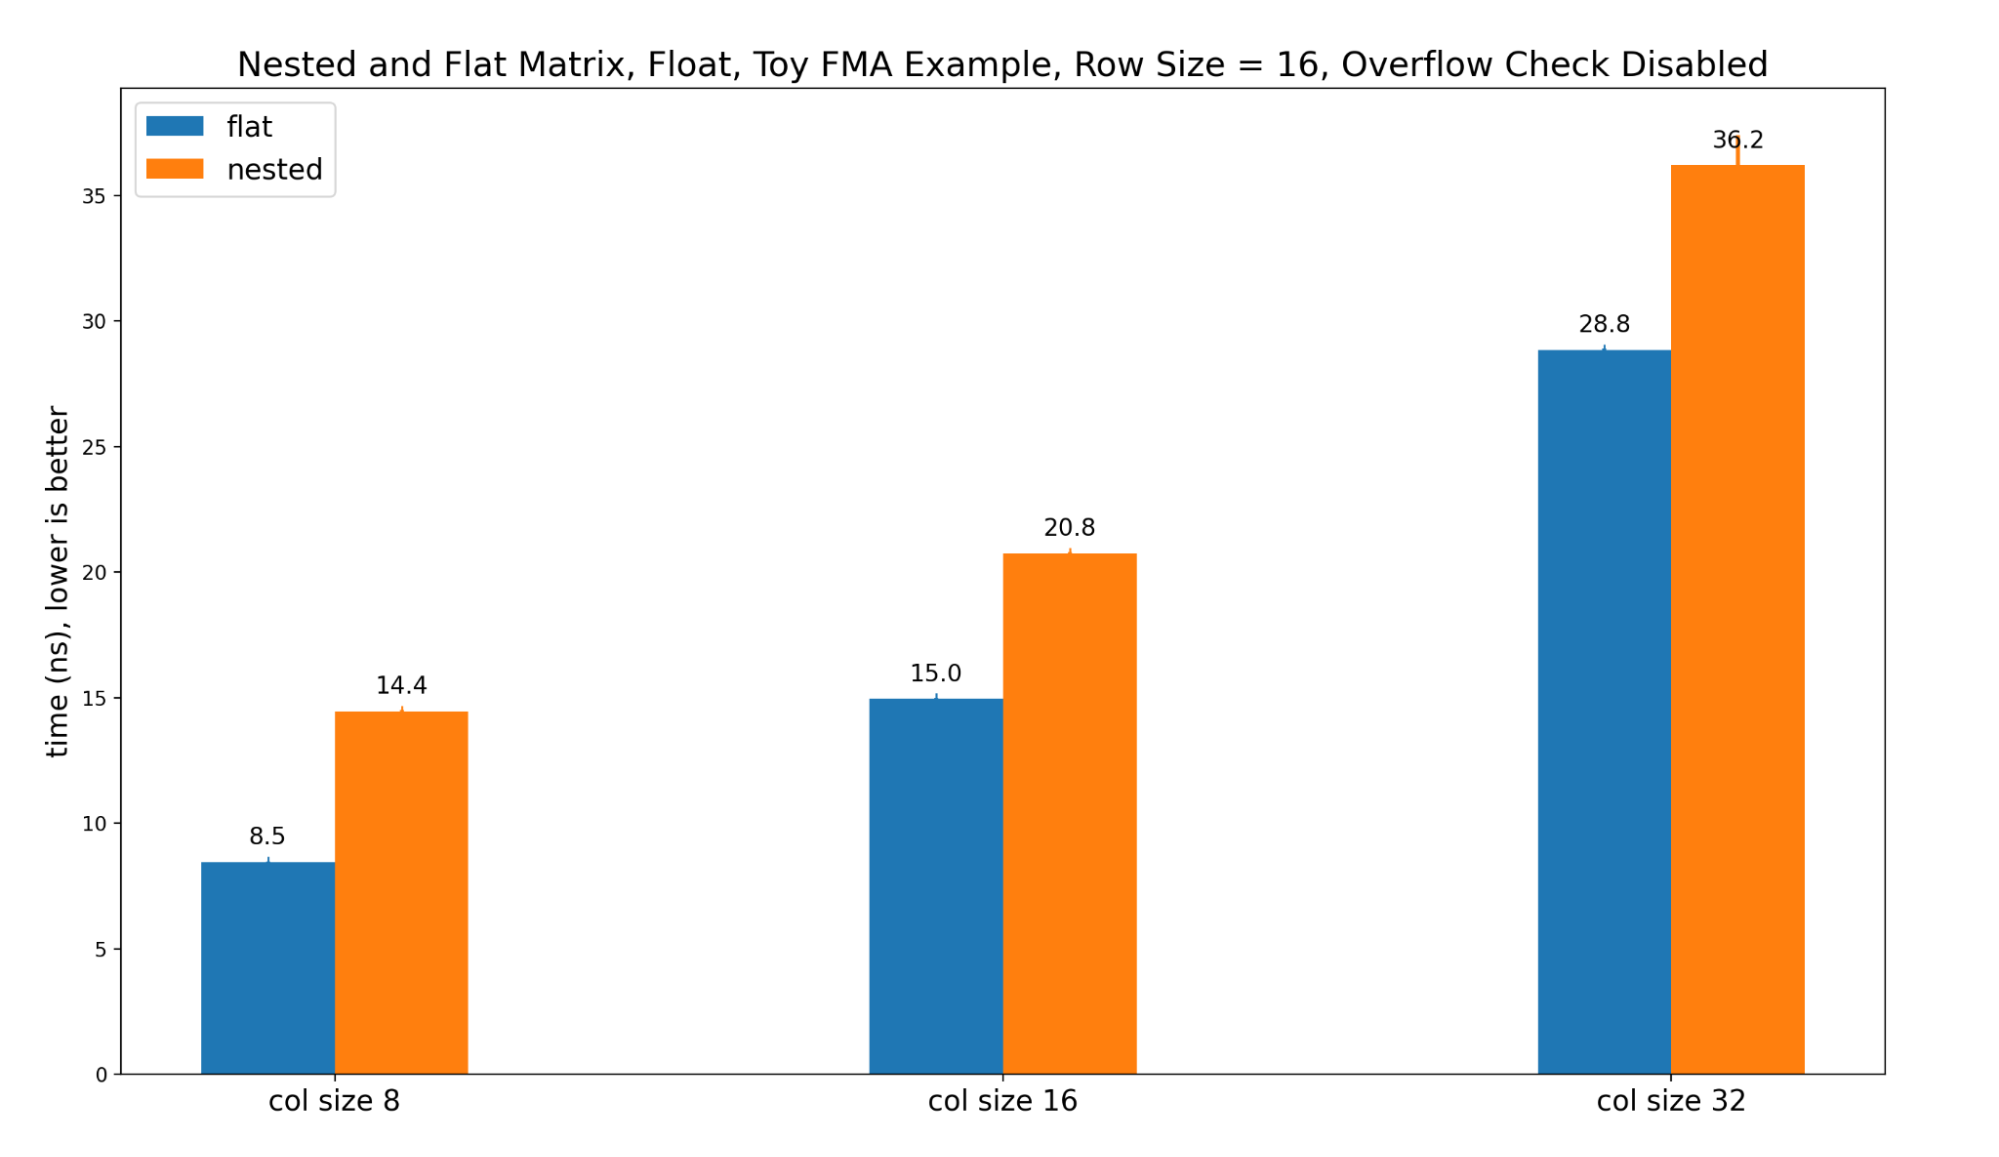
\includegraphics[width=\linewidth]{image/nested-flat.jpg}
    \caption{\hl{TODO: write caption}}
    \label{fig:nested-flat}
\end{figure}


\section{Matrix element data type}


\subsection{Width}
\label{sec:width} 
Since the numbers stored in the matrix are almost always less than 10 bits,
using shorter data types can be more advantageous than longer ones because they
allow more numbers to be packed into a single vector register (Figure
\ref{archtable}). The number of instructions can be cut by half when data width
is reduced to half, and less instruction count always leads to less execution
time. Given that the Zen4 micro-architecture provides approximately same amount
of execution units for both integers and floating points, it is reasonable to
estimate that the execution time is inversely proportional to the bit width of
data type. As confirmed in Figure \ref{bench_datatype}, when overflow is
ignored, \dtint{} and \dtfloat{} costs nearly same amount of time, while
\dtint{} and \dtdouble{} costs double the amount of time than \dtshort{} and
\dtfloat{} respectively.


\begin{figure}[H]\captionsetup{name=Figure}
    \captionsetup{justification=centering}
    \begin{center}
        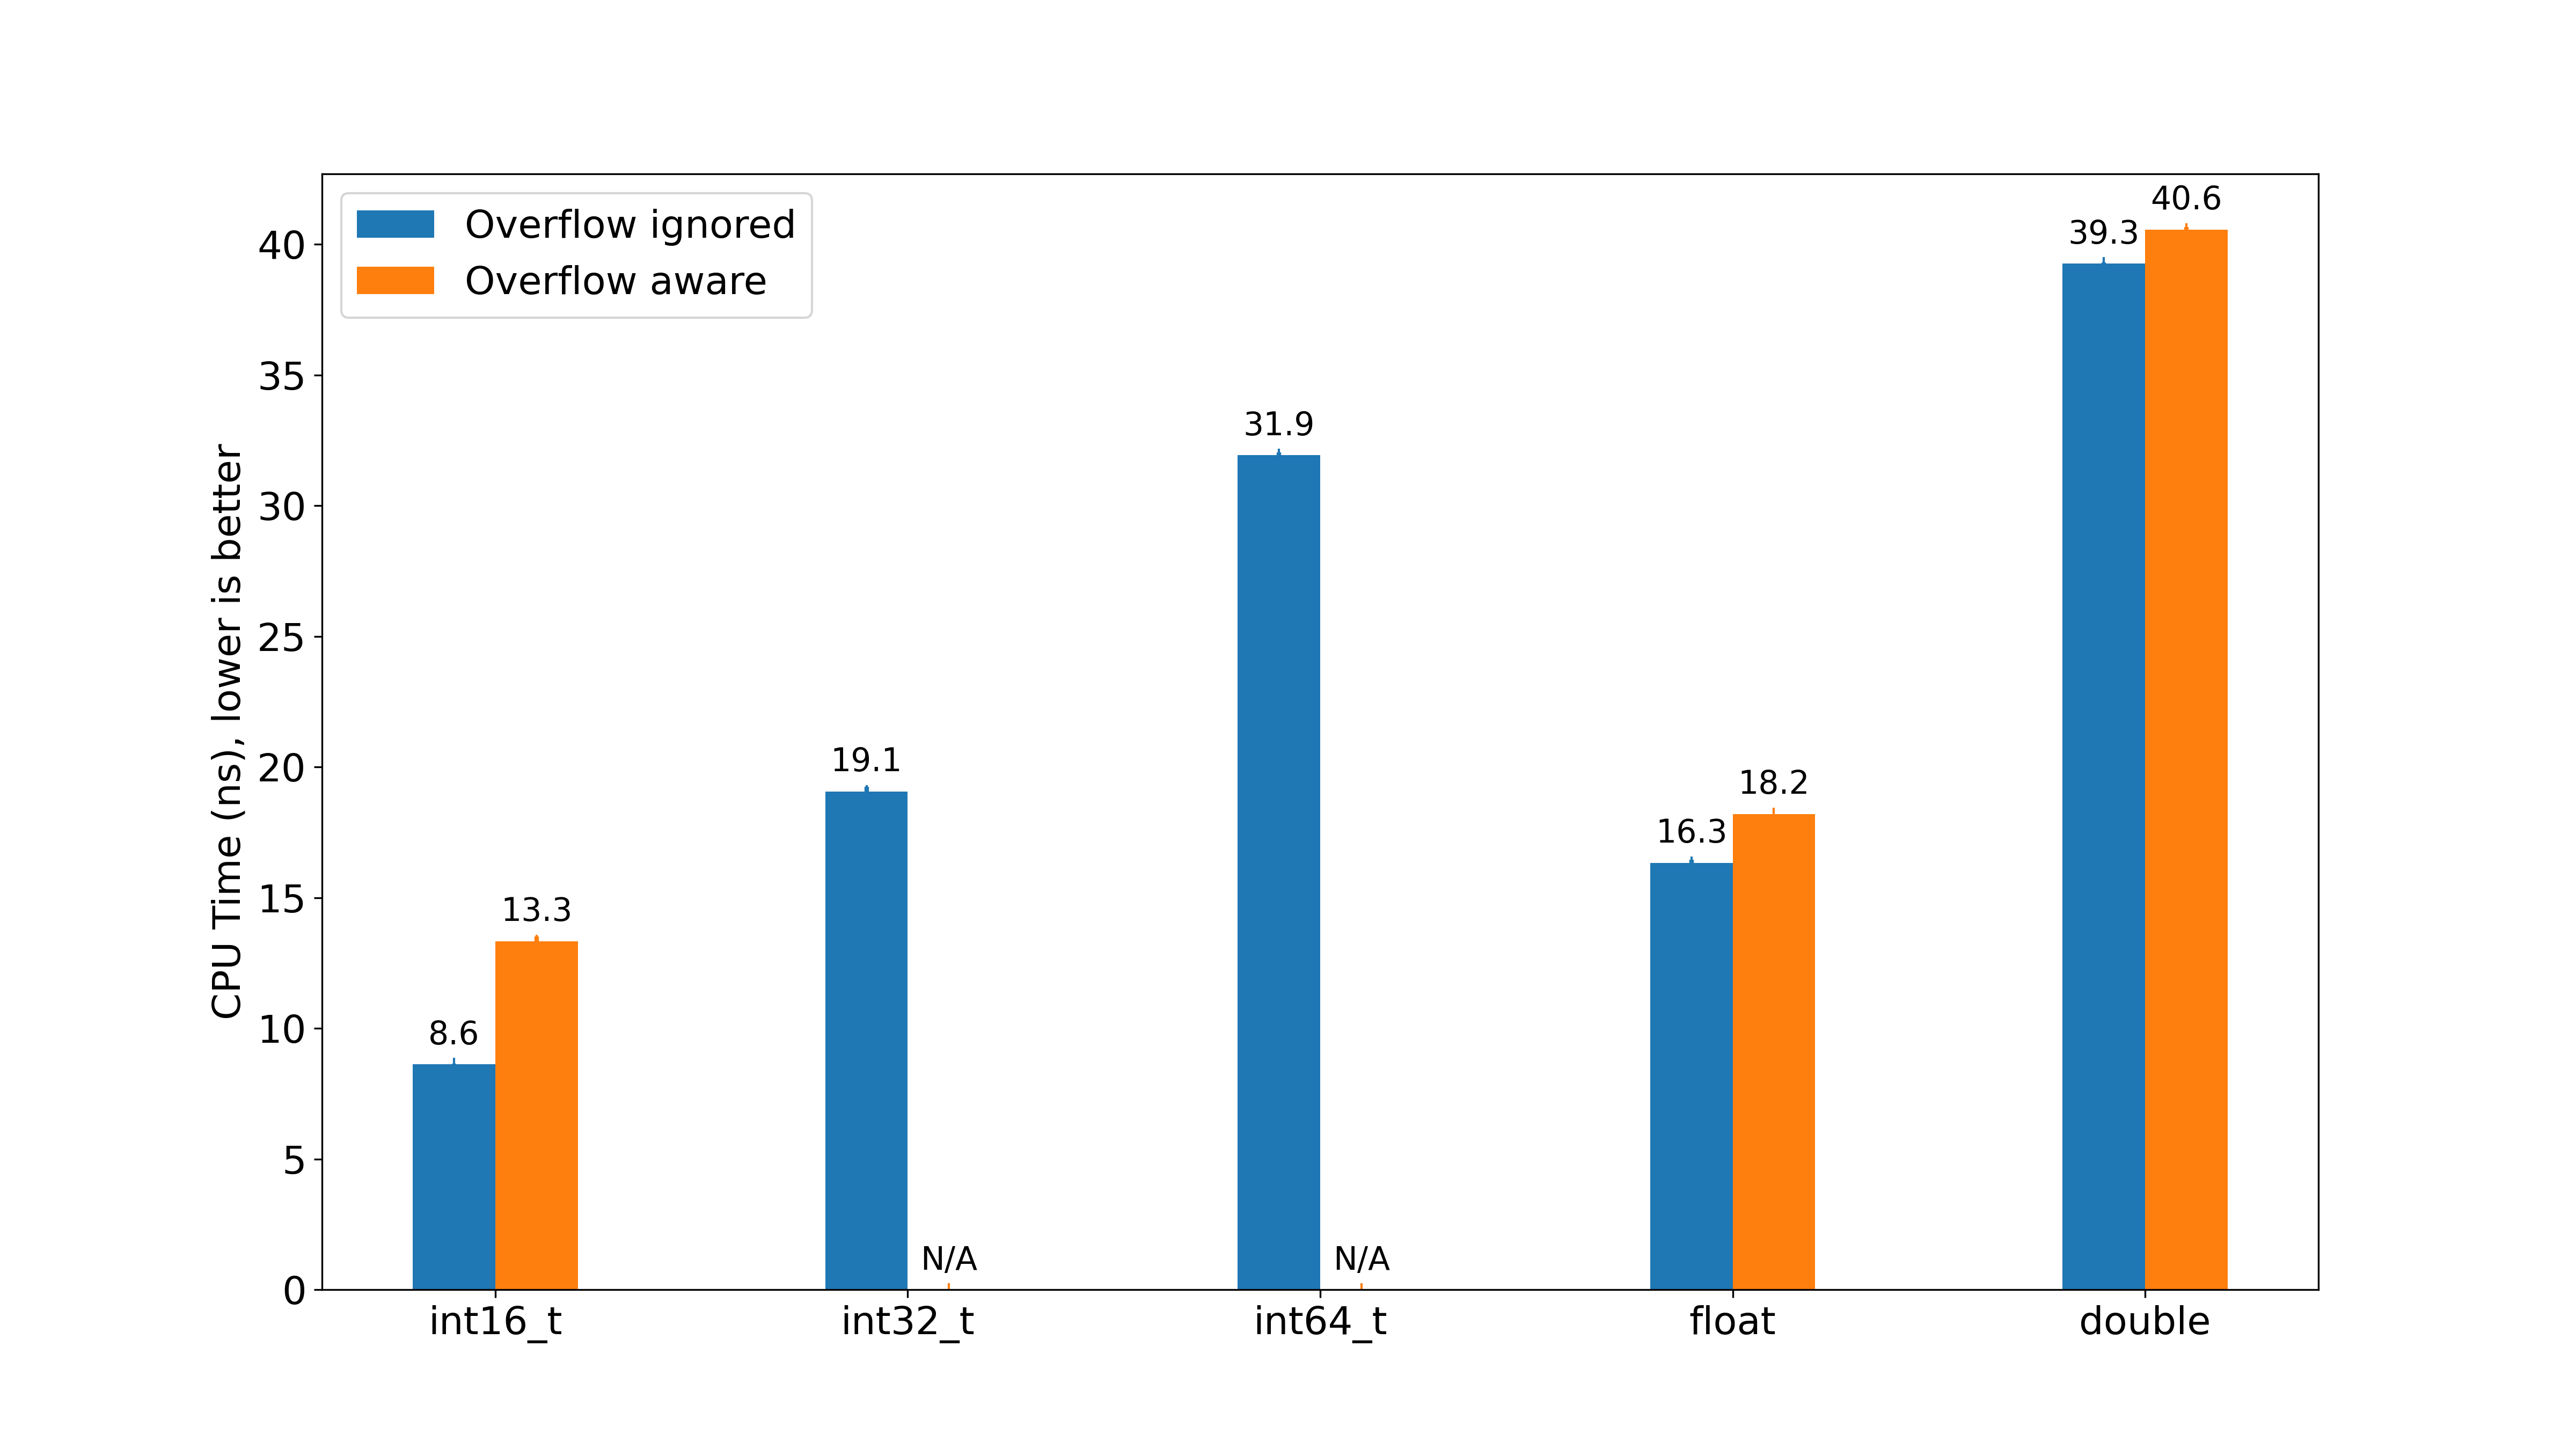
\includegraphics[width=\linewidth]{image/bench_datatype.png}
    \end{center}
    \caption{It is difficult to check overflow for vectorized \dtint{} and
    \dtlong{}, therefore their runtime are unavailable. }
    \label{bench_datatype}
\end{figure}

% \begin{figure}[H]
%     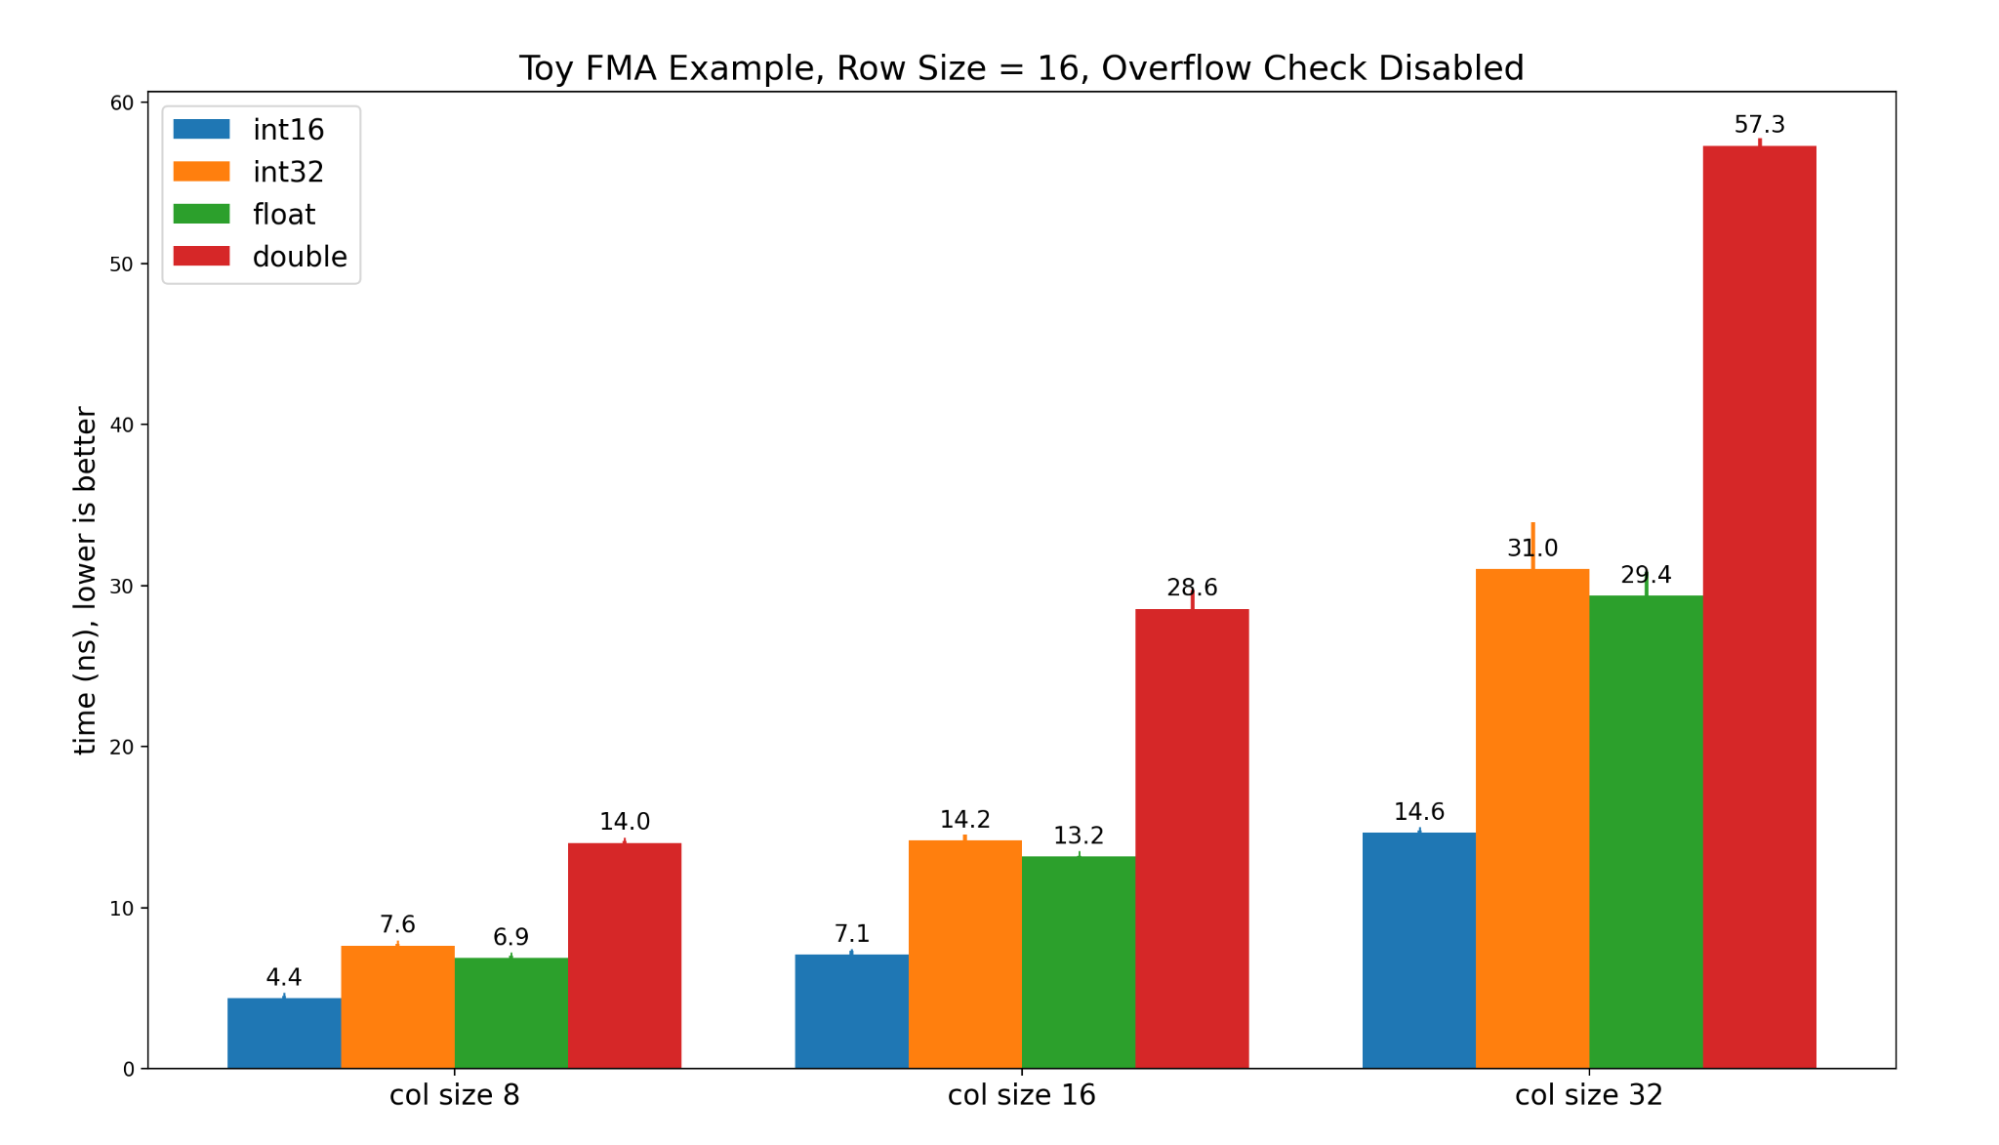
\includegraphics[width=\linewidth]{image/col8-col16-col32-i16-i32-f32-f64.png}
%     \caption{\hl{TODO: write caption}}
%     \label{fig:col8-col16-col32-i16-i32-f32-f64}
% \end{figure}

% \hl{TODO: fix Table number}
\begin{figure}[H]\captionsetup{name=Figure}
\captionsetup{justification=centering}
    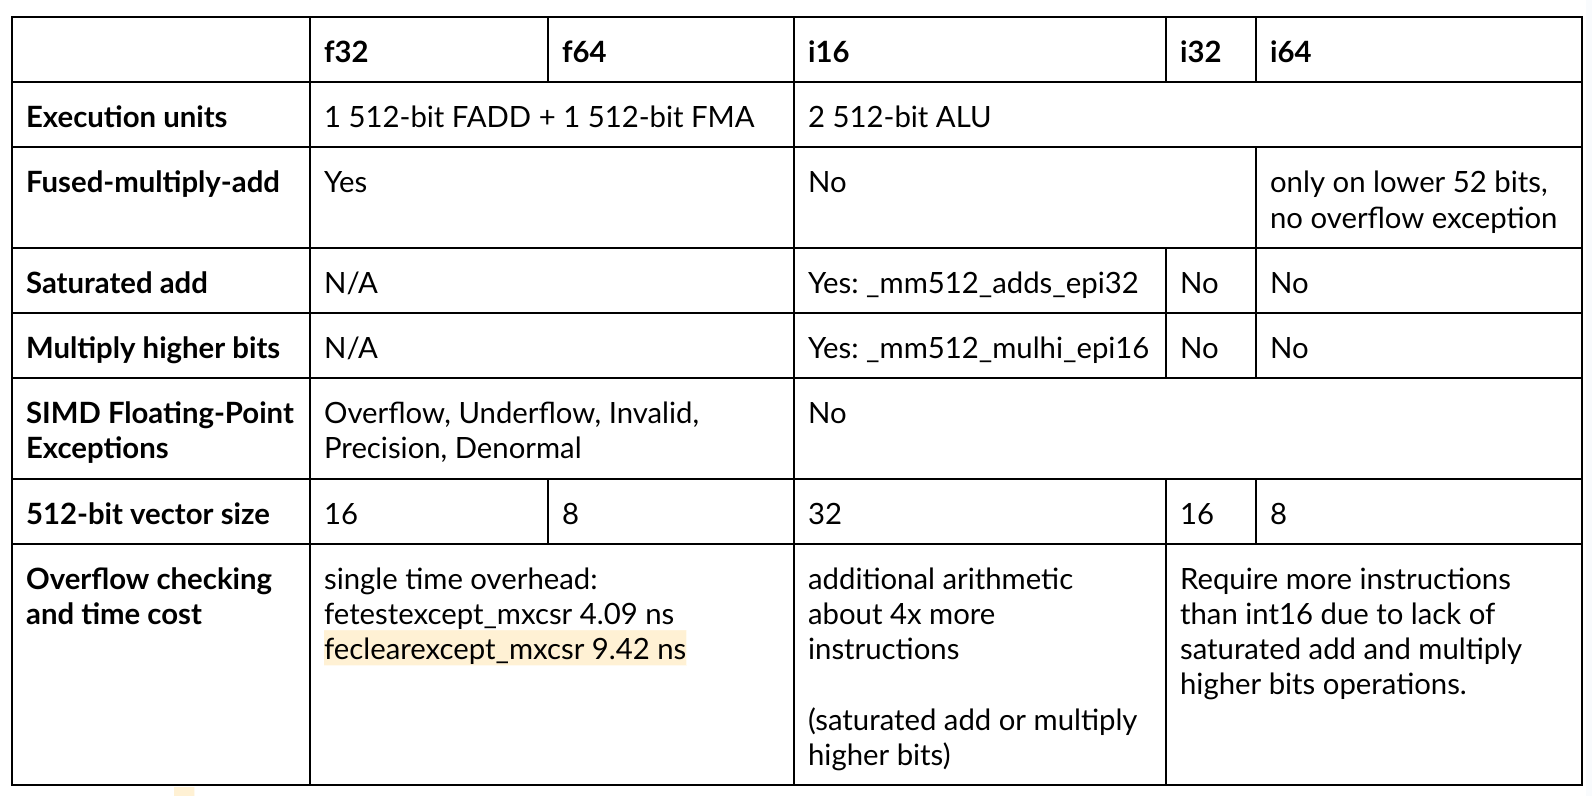
\includegraphics[width=\linewidth]{image/arch-table.png}
    \caption{A summary of features provided by the Zen4 micro-architecture for
    different data types~\cite{Zen4Critique}~\cite{Zen2ChipWiki}.}
    \label{archtable}
\end{figure}

\subsection{Overflow checking for integers}
\label{sec:overflow-int}

The x86-64 micro-architecture provides the \texttt{seto} instruction to set some
byte to \texttt{1} if overflow occurred as a result of integer arithmetic.
However \texttt{seto} only works for scalar operations, there does not exist
instruction or status register to indicate whether a previous vector add or
multiply instruction produces overflown results or not. Therefore, overflow has
to be checked manually by some additional vector instructions, this would slow
down the computation to some extent. Or alternatively or arithmetics have to be
carried out on each element individually in a scalar manner,resulting in even
worse performance. 


% One advantage of using \dtshort{} is that it can be used with AVX-512's
% saturated add and multiply higher bits vector instructions, which are listed in
% Table \ref{archtable}. This allows for the creation of vectorized code that
% takes overflow into account and is therefore more efficient. However, it should
% be noted that there are no equivalent instructions for \texttt{int32_t} and
% \texttt{int64_t}.

One advantage of \dtshort{} is that it can be used with \texttt{AVX-512}'s
saturated add and multiply higher bits vector instructions (Figure 
\ref{archtable}), making it possible and convenient to write vectorized and
overflow-aware code. However, Zen4's implementation of \texttt{AVX-512} extension does
not provide equivalent instruction for \dtint{} or \dtlong{},
and therefore must be processed as scalar values.
% When the
% result of a conventional add does not match the result of a saturated add, or
% when multiplying for the higher 16 bits gives non-zero results, it implies an
% overflow. 


\subsubsection{Implementation of vectorized \dtshort{} overflow checking}
\label{sec:i16-overflow-checking}
By comparing the result of a conventional addition and saturated addition, it
indicates whether an addition has gone overflown or not. In case of overflow,
with saturated add, the result always retains at the maximum possible value of
\dtshort{}: \texttt{0x7FFF}, while the result of a conventional add is
always smaller, because the overflowed output from conventional addition can't
go all the way around and become \texttt{INT16\_MAX} again. In the two's
complement binary form for integer, the overflow sum is "trapped" in the
negative number space. For example: 
\begin{verbatim}
INT16_MAX + 1 = INT16_MIN = -32768, 
INT16_MAX + 2 = -32767, 
...
INT16_MAX + INT16_MAX = -2, 
\end{verbatim}

For multiplication, as two 16-bit numbers produces 32-bit products but only
lower 16 bits can be stored, overflow can be detected by checking whether any of
the upper 16 bits are set. 

Inspecting these approaches from a instruction-level perspective (Table
\ref{table:i16-instr}), when overflow is ignored, both add and multiply takes 1
instruction, 
\hlc[pink]{\texttt{vpaddw}}\footnote{Vector add for \dtshort{}} 
and 
\hlc[pink]{\texttt{vpmullw}}\footnote{Vector multiply lower half bits for \dtshort{}}. 
To obtain and process overflow-related
information, an additional computation instruction
\hl{\texttt{vpaddsw}}\footnote{Vector saturated add for \dtshort{}}
or
\hl{\texttt{vpmulhw}}\footnote{Vector multiple higher half bits for \dtshort{}} 
is required, followed with 2 or 3 comparison, shuffling and branch instructions:
\hlc[cyan!60]{\texttt{vpsraw}}\footnote{Shift packed data right arithmetic},
\hlc[cyan!60]{\texttt{vpcmpneqw}}\footnote{Compare packed data for equal}
and 
\hlc[cyan!60]{\texttt{kord}}\footnote{Bitwise logical OR masks}. 
By enabling
overflow checking, it brings 4 to 5 times more instruction count and 65\% more
runtime~\cite{FPL2}.

\begin{center}
\begin{table}[ht]
\centering
\captionsetup{justification=centering}
\begin{tabular}{  c  L{5.5cm} L{5.5cm}  } 
     & Addition & Multiplication \\ 
    \midrule
        Ignored 
    & 
        \hlc[pink]{\texttt{vpaddw \%zmm4,\%zmm2,\%zmm3}} 
    &
        \hlc[pink]{\texttt{vpmullw \%zmm1,\%zmm3,\%zmm2}} \\
    \midrule
        Enabled 
    &
        \hlc[pink]{\texttt{vpaddw \%zmm4,\%zmm2,\%zmm3}}
        \hl{\texttt{vpaddsw \%zmm2,\%zmm4,\%zmm2}}
        \hlc[cyan!60]{\texttt{vpcmpneqw \%zmm3,\%zmm2,\%k1}}
        \hlc[cyan!60]{\texttt{kord \%k1,\%k0,\%k0}}
    &  
        \hlc[pink]{\texttt{vpmullw \%zmm1,\%zmm3,\%zmm2}}
        \hl{\texttt{vpmulhw \%zmm1,\%zmm3,\%zmm3}}
        \hlc[cyan!60]{\texttt{vpsraw \$0xf,\%zmm2,\%zmm5}}
        \hlc[cyan!60]{\texttt{vpcmpneqw \%zmm3,\%zmm5,\%k1}}
        \hlc[cyan!60]{\texttt{kord \%k0,\%k1,\%k0}} \\
  \end{tabular}
\caption{For vectorized \dtshort{}, this table highlights the difference in
terms of instruction count when overflow checking is enable or disabled.
\hlc[pink]{Pink} instructions are required in both versions. Overflow information
are provided by \hl{yellow} and 
\hlc[cyan!60]{cyan} instructions. }
  \label{table:i16-instr}
\end{table}
\end{center}
\subsubsection{Implementation of scalar \dtint{} and \dtlong{}
overflow checking} 

\hl{TODO:Not sure if this section is necessary or not?}

Clang's language extension provides functions to perform overflow-checked
integer arithmetics: 
\begin{VerbatimCompact}
bool __builtin_add_overflow (type1 x, type2 y, type3 *sum);
bool __builtin_mul_overflow (type1 x, type2 y, type3 *prod);
\end{VerbatimCompact}
These functions take three arguments: \texttt{x} and \texttt{y} are the two
input operands, and \texttt{sum} or \texttt{prod} is a pointer to the variable
that will hold the result of the addition or multiplication. The return value of
these functions is a boolean that indicates whether an overflow occurred during
the operation.


\subsection{Overflow checking for floating points}
\label{sec:overflow-float}
To detect floating point overflow or imprecision, one approach is to enable
floating point imprecision as a trap, then upon overflow, the interrupt \sigfpe{}
is raised and the PC (program counter) will be redirected to its handler. The
method can be programmed by using useful functions from the \texttt{fenv}
library as follow~\cite{fenvlib}:
\begin{verbatim}
void signal_handler(int signal) {
    // handle fpe
}

void function() {
    std::signal(SIGFPE, signal_handler);
    std::feclearexcept (FE_ALL_EXCEPT);
    feenableexcept (FE_INEXACT | FE_INVALID);
    // do something
    fedisableexcept (FE_INEXACT | FE_INVALID);
}
\end{verbatim}

In the \texttt{function()} block, first the \texttt{std::signal()} function is
called to register the signal handler function for the \sigfpe{} interrupt. Next,
the \texttt{feclearexcept()} function is called to clear any previously set
exception flags in the status register. Then, \feinexact{} and \feinvalid{} is
passed to the \texttt{feenableexcept()} function to enable inexactness and
invalid exceptions. Once the floating-point exceptions are enabled, some
computation can be performed. If some operation produces an inexact or invalid
floating point number, \sigfpe{} is raised and a call to
\texttt{signal\char`_handler} is triggered. After the computation is completed,
the \texttt{fedisableexcept()} function is called to disable the previously
enabled exceptions. 

But it is difficult to recover back from \sigfpe{}. By design, the propose usage
of \sigfpe{} is to do some cleanup in the handler function, then exit the program
gracefully. If the handler does not exit the program, after returning from the
handler, the PC always points back to the instruction that caused \sigfpe{} and
triggers \sigfpe{} again! However the goal is to discard the current progress and
continue the program by using the LargeInteger algorithm. Although there could
be potential workarounds, such as modifying the call stack and changing the
return address, but implementing these solutions can be challenging, and
introduces significant complexity to the codebase.

Alternatively we may read status registers and check if the imprecision bit is
set: 
\begin{verbatim}
bool function(matrix & tableau) {
    std::feclearexcept (FE_ALL_EXCEPT);
    if (fetestexcept(FE_INEXACT | FE_INVALID)) {
        // false for overflow, will be handle by its caller
        return false; 
    } return true; // true for safe
}
\end{verbatim}

Instead of registering floating point imprecision as interrupts, it clears the
floating point status register with \texttt{feclearexcept()} and reads it
afterwards using the
\texttt{fetestexcept()} function, to check whether imprecision has ever occurred
in previous computations. It then returns a boolean value to notify its caller
whether or not the test for floating-point exceptions is positive, \texttt{true}
for safe and \texttt{false} for overflown. In case of returning \texttt{false}, 
the caller will retry computation using \texttt{LargeInteger} accordingly. 



\subsubsection{Evaluation}
In x86\_64 there are two status registers for floating points, the legacy x87
status register for traditional scalar floating point operation, and the modern
\mxcsr{} register for \texttt{SSE} or \texttt{AVX} instructions. The source code
of the library function \texttt{fetestexcept} indeed manipulates both registers
\cite{fenvlib}: 
\begin{verbatim}
int fetestexcept(int excepts) {
    unsigned short status;
    unsigned int mxcsr;

    excepts &= FE_ALL_EXCEPT;

    /* Store the current x87 status register */
    __asm__ volatile ("fnstsw %0" : "=am" (status));

    /* Store the MXCSR register state */
    __asm__ volatile ("stmxcsr %0" : "=m" (mxcsr));

    return ((status | mxcsr) & excepts);
}
\end{verbatim}


In the vectorized floating point scenario, the instruction for x87 status
register is unnecessary and only the \mxcsr{} register should be concerned. The
hot loop is completely vectorized, and clang dispatches 128-bit \texttt{SSE}
instructions for occasional scalar operations. This is because the \texttt{SSE}
execution units can handle both single and double precision floating point
arithmetic natively, whereas the legacy x87 floating-point instructions operates
on an 80-bit internal format, requiring additional conversions and delay. Using
\texttt{SSE} instructions reduces register pressure as well. The \texttt{SSE}
units can leverage 16 \xmm{} registers, but for x87 units there are only 8
floating point registers available. There could be even 32 \xmm{} registers if
such extension is implemented in the micro-architecture~\cite{x87-bad}. 

The benchmark, as illustrated in Figure \ref{plot_fenv}, evaluates the
performance of \texttt{fenv} functions alongside their respective revised
versions. The modifications involves restricting operations solely to the
manipulation of either the x87 status register or the \mxcsr{} register. It
indicates that it is significantly faster if we remove x87 status register
related operations. 

\begin{figure}[H]\captionsetup{name=Figure}
    \captionsetup{justification=centering}
    \begin{center}
    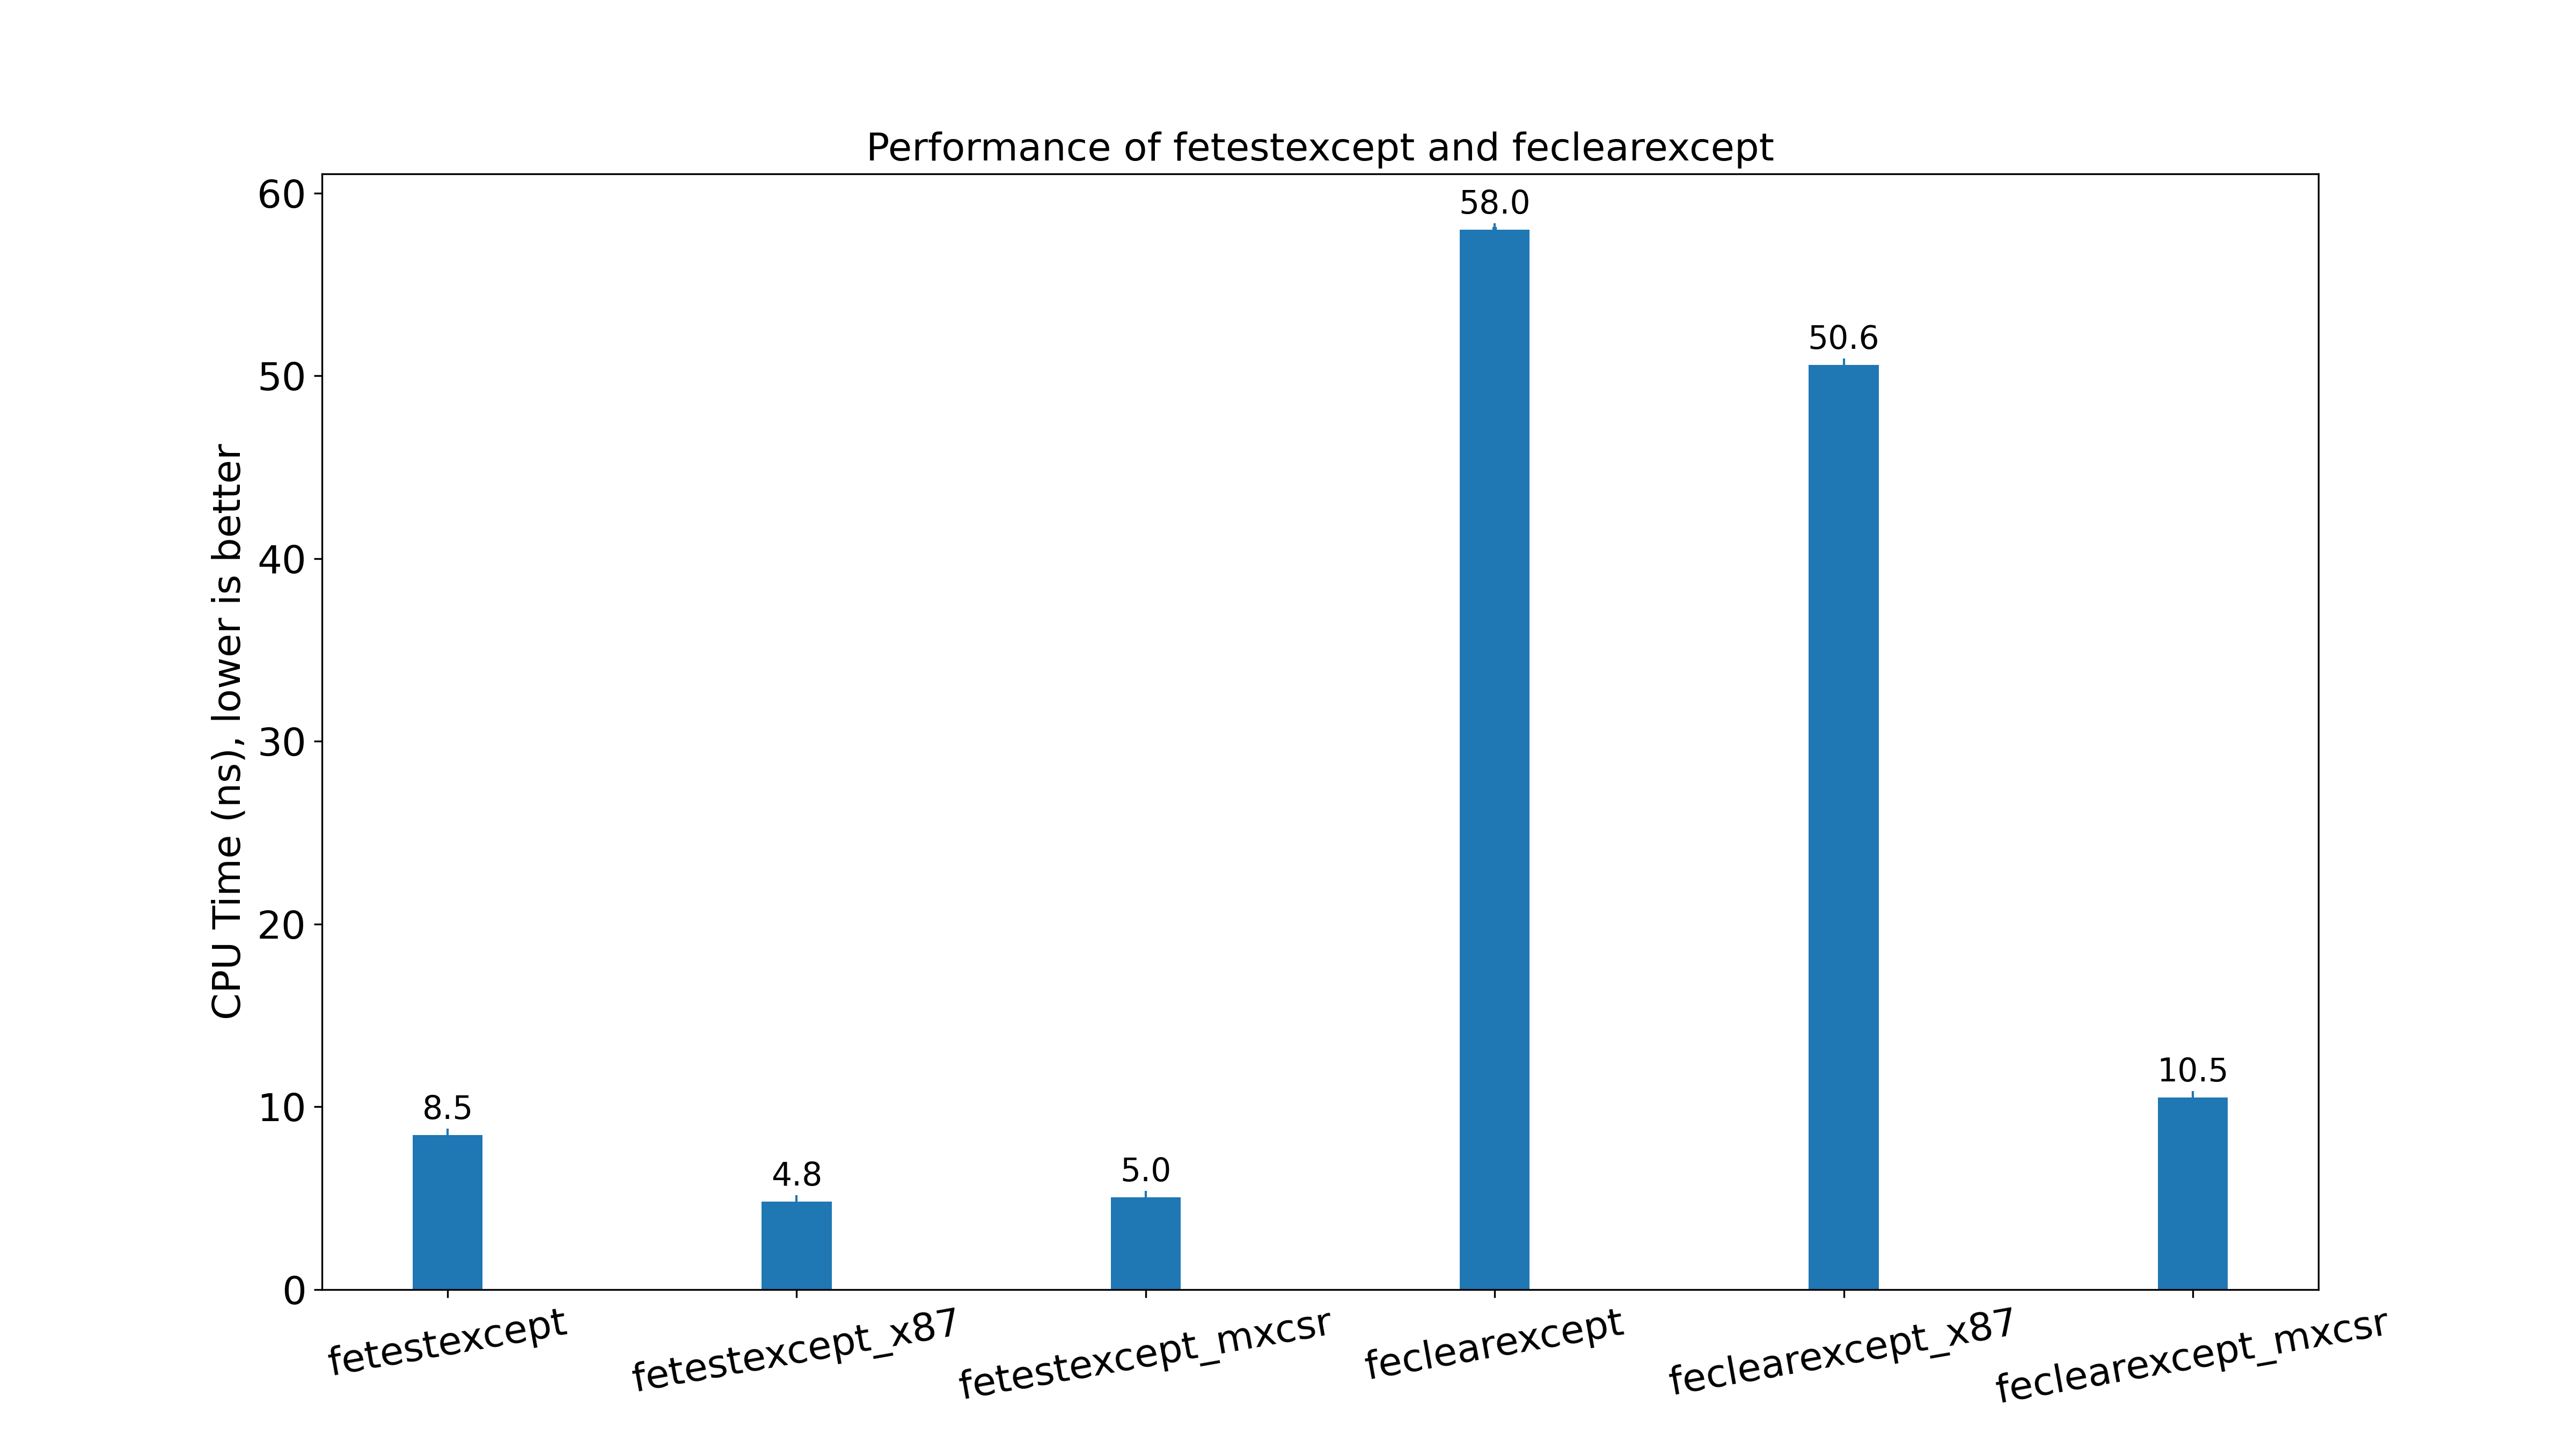
\includegraphics[width=\linewidth]{image/bench_fenv.png}
    \end{center}
    \caption{Performance of the \texttt{fetestexcept()} and \texttt{feclearexcept()}
    function from \texttt{cfenv} library. \hl{TODO:}}
    \label{plot_fenv}
\end{figure}
\normalsize

\subsection{Comparing \dtshort{} and \dtfloat{}}

Section \ref{sec:width}, \ref{sec:overflow-int} and \ref{sec:overflow-float}
have concluded that \dtshort{} is superior than any other integer data types and
\dtfloat{} is better than \dtdouble{}. 

% even
% though \dtshort{} is the fastest on this particular matrix size

Benchmark (Figure \ref{bench_datatype}) on the toy example reveals that
\dtshort{}'s spends a considerably higher percentage of runtime on overflow
checking, compared with the floating point data types. This is consistent with
the reasoning from previous chapters, where overhead for \dtfloat{} is a
one-time expense, but for \dtshort{} it is always a portion of the total
runtime. 

Note that even though \dtshort is faster than \dtfloat in this benchmark, it is
not sound to conclude that the \pivot{} function implemented in \dtshort
will be faster than \dtfloat. The toy example is different from the \pivot
function in many aspects, for example, number of memory load operations. In case
of the actual \pivot{} function, float may potentially outperform int16. 

% \begin{verbatim}
% bool function(matrix & tableau) {
%     // do something
%     if (fetestexcept(FE_INEXACT | FE_INVALID)) {
%     return false; // false for overflow, will be handle by its caller
%     } return true; // true for safe
% }

% void caller(){
%     ...
%     std::feclearexcept (FE_ALL_EXCEPT);
%     if (!function(tableau)) {
%         // overflow! retry with bigger precision algorithm
%     }
% }
% \end{verbatim}


\chapter{Implementation and Optimization of \pivot{}}

\section{Matrix-wise transprecision}
Transprecision techniques can be implemented at different levels of scale, such
as element-wise, row-wise, and matrix-wise. The vectorized versions of \pivot{}
are implemented using the matrix-wise transprecision style. For \dtfloat{},
the \mxcsr{} register accumulates information regarding previous occurrences of
overflow and imprecision, until it is cleared manually. 

The element-wise method is not suitable in this scenario, as it defeats the
purpose of vectorization. The row-wise method is not chosen either, due to that
overflow is not likely to occur and the matrix is small. Reading the \mxcsr{}
can be considered as a expensive operation, comparing to the time spent on
pivoting through the entire matrix. Avoiding wasted arithmetic instructions
after overflow at the cost of more \mxcsr{} reads is not a cost-effective
trade-off.

Even though the \pivot{} function using \dtshort{} was implemented using the
row-transprecision approach in previous works~\cite{FPL2}, it is modified to
match with the matrix-wise transprecision style, in order to control differences
between the \dtfloat{} counterpart. After the overflow checking instructions,
instead of a branch instruction pointing to the overflow handler, the boolean
operator OR is applied between that overflow checking result register and a
overflow flag. 


\section{Double buffering}

Double buffering is a powerful technique to address the issue of data pollution
caused by overflown data. When matrix-wise computing is carried out, a potential
overflow can contaminate the input matrix and write meaningless results into it.
It is difficult to recover from overflown results, making it impossible to
dispatch the same input matrix to a algorithm of higher precision and defeating
the purpose of transprecision computing.

Double buffering addresses this challenge by allocating two distinct pieces of
memory, one for the input matrix and the other for output matrix. The input
matrix is read-only, while the output matrix allows both reading and writing.
This separation of data storage ensures that the input matrix remains unpolluted
by overflown data and that any potential overflow is encapsulated within the
separate output matrix. 

While making a copy of the input matrix is a simple and easy solution for
protecting the original data from pollution, double buffering is a superior
technique due that it does not introduce additional memory operations. With
double buffering, every operand requires a load operation from the input matrix,
and every result takes a store operation to be written into the output matrix.
This is the minimal amount of memory operation required for arithmetics. Zen4 is
capable of loading one \zmm{} vector per cycle and storing one \zmm{} vector per two
cycles. In comparison, it can do two multiplication or addition of \zmm{}
vectors every cycle. The discrepancy in throughput between computing and IO
suggests that memory copy very expensive and inefficient. 

\section{Alignment}
In the Listing \ref{table:vec-fma-float} and Listing \ref{vec-fma-int}, the
assembly for load and store are \texttt{vmovups} and \texttt{vmovdqu64}. 
\texttt{vmovups} for
``Move Unaligned Packed Single-Precision Floating-Point Values''~\cite{vmovups},
and \texttt{vmovdqu64} for 
``Move Unaligned Packed Integer Values''~\cite{vmovdqu64}. 

Unaligned load may bring potential performance impacts. When accessing memory,
the CPU retrieves data from the main memory or cache in units of cache lines. On
Zen4 the size of cache line is 512-bits, exactly the size of a \zmm{} register
\cite{AMDManual}. Alignment guarantees that a single cache line can cover a
vector register. Otherwise, a \zmm{} register might be spitted on two cache lines.
Both cache lines of 1028 bits have to be requested from the memory, then
performs a shift to extract the desired 512 bits~\cite{Unaligned}.  

To address this issue, an aligned allocator is given to the constructor of
\texttt{std::vector} when initializing a matrix~\cite{FPL2}. 
 The compiler is capable of recognizing alignment
and issue aligned load instructions \texttt{vmovdqa} or \texttt{vmovaps}
accordingly. 

\section{Reduce number of matrix index computation}
\label{sec:optmz-get-index}

Section \ref{sec:mat-structure} discussed the benefits of using a single
\texttt{std::vector} to represent a matrix. Given arbitrary row and column, the
item of the matrix can be found in the array by computing the index:
\texttt{column count * row + column}. The matrix data structure can be further
optimized if the number of index computations can be reduced. By placing the
pivot row as the first row in the matrix, it is only required to compute the
address once for the first element of the matrix, then every subsequent item can
be indexed by incrementing the address. 

% \subsection{Loop unrolling}



\section{Vector size specialization}

A \ymm{} register can pack 8 \dtfloat{}s, and a \zmm{} register can pack 16
\dtfloat{}s (Figure \ref{archtable}). Since most of the input matrices have less
than 20 columns (\ref{sec:presburger}), representing a row with 2 \zmm{} vectors
introduces padding waste of at least 12 \dtfloat{}s, but using 3 \ymm{}
registers for a row reduces the minimal padding size to 4 \dtfloat{}s. 

To avoid such padding waste, my implementation \pivot{} function with \dtfloat{}
is specialized for 4 different column size, using \ymm{} and \zmm{} registers to
represent a row. There are 16 combinations in total:
\vspace*{-4mm}
\begin{table}[H]
\centering
\captionsetup{justification=centering}
% \begin{tabular}{lll}
    %    & \ymm{} register count & \zmm{} register count \\
    % Column $\leq$ 8  & 1   & 1   \\
    % Column $\leq$ 16 & 2   & 1   \\
    % Column $\leq$ 24 & 3   & 2   \\
    % Column $\leq$ 32 & 4   & 2  
    % \end{tabular}
\begin{tabular}{lllll}
    1. & \dtfloat{}, Column $\leq$ 8  & 1 \ymm{} register  & or &  1 \zmm{} register   \\
    2. & \dtfloat{}, Column $\leq$ 16 & 2 \ymm{} registers & or & 1 \zmm{} register   \\
    3. & \dtfloat{}, Column $\leq$ 24 & 3 \ymm{} registers & or & 2 \zmm{} registers   \\
    4. & \dtfloat{}, Column $\leq$ 32 & 4 \ymm{} registers & or & 2 \zmm{} registers  \\
    \hline
    5. & \dtshort{}, Column $\leq$ 8  & 1 \ymm{} register  & or &  1 \zmm{} register   \\
    6. & \dtshort{}, Column $\leq$ 16 & 1 \ymm{} registers & or & 1 \zmm{} register   \\
    7. & \dtshort{}, Column $\leq$ 24 & (unimplemented) & or & 1 \zmm{} registers   \\
    8. & \dtshort{}, Column $\leq$ 32 & (unimplemented) & or & 1 \zmm{} registers  
    \end{tabular}
\end{table}
\vspace*{-8mm}

\begin{figure}[H]
    \begin{center}
        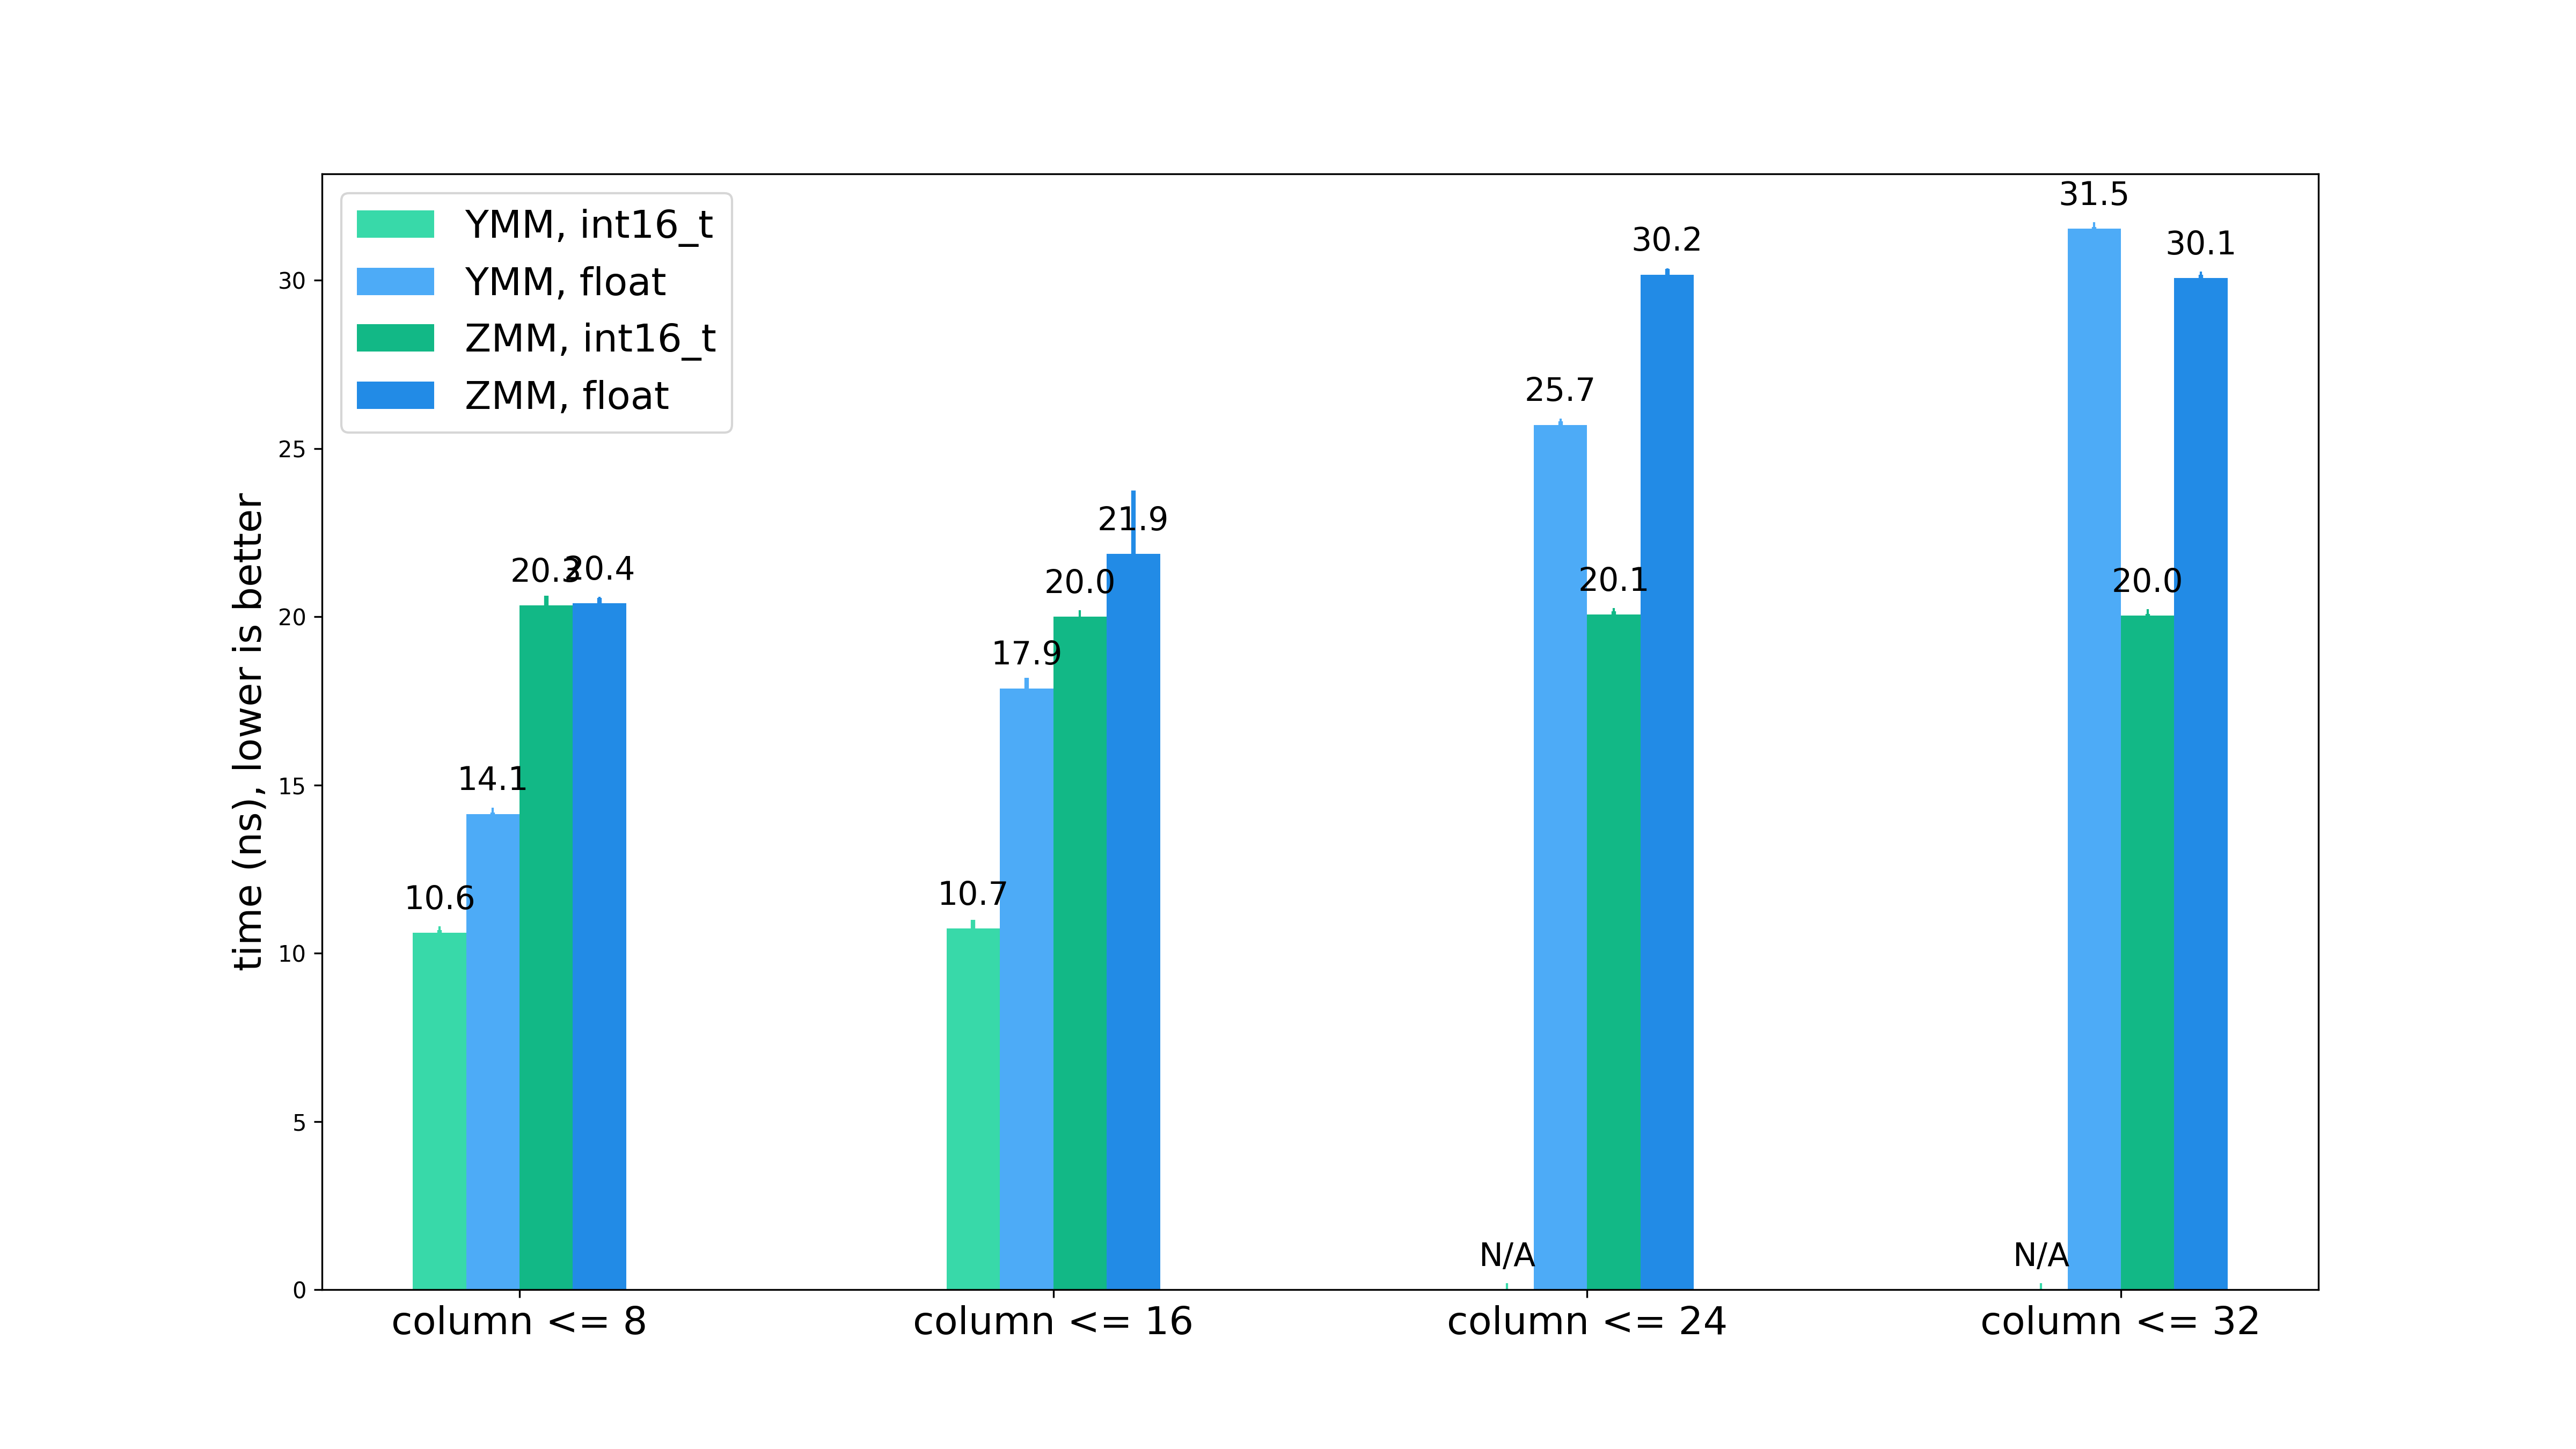
\includegraphics[width=\linewidth]{image/specialize-i16-f32.png}
        % 
\includegraphics[width=50mm]{image/turtle.png}
    \end{center}
    \caption{\hl{TODO: write caption}}
    \label{fig:specialization}
\end{figure}

\section{Evaluation}

% It is found that for matrices with small column sizes that fits 

Figure \ref{small-val-low-dim} shows that 95\% most of the matrices have less 20
columns while 75\% of the matrices have more than 18 columns~\cite{FPL1}. Thus
the number of columns of a matrix is very likely to be between 16 and 24, and the 
perform 

% unfortunately \dtfloat{} does not provide a performance advantage over \dtshort{}.


    % Specifically, \dtfloat{} takes 26 ns, while \dtshort{} completes 6 ns ahead.
    % Nevertheless, both of them significantly outperform the upstream scalar
    % implementation, which renders the 6 ns gap trivial. 
    % Additionally, \dtfloat{} offers substantial compatibility advantage
    % over \dtshort{} for vast amount of non-\texttt{AVX-512} platforms. 


\chapter{Conclusion and Future work}

\dthalf{} is a 16-bit floating point data structure, consistent of 1-bit sign,
5-bit exponent and 10-bit mantissa (Figure \ref{fig:ieee-f16}). The \dthalf{}i{}
data type can be defined accordingly, and overflow would not occure for xx\% of
the cases. 

Now \dthalf{} has already been supported widely on GPUs for AI applications. It
provides performance benefits over higher precision floating point formats, for
the exact same reason that extra precisions are a waste of resources, and more
number can be computed once with a a shorter data type. If 16-bit floating point
is integrated into future \texttt{AVX} extensions, it would further improve the
performance of \pivot{}. It is expected to be slightly slower then the \dtshort{}
overflow-ignored version, and the runtime can be reduced to about 50\% comparing
to the \pivot{} function implemented using \dtfloat{} in this report.

\begin{figure}
    \begin{center}
    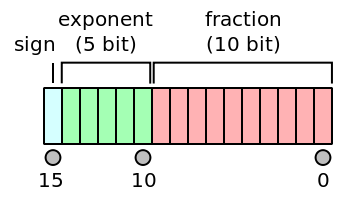
\includegraphics[width=50mm,scale=0.1]{image/ieee-f16.png}
    \end{center}
    \caption{IEEE 754 half precision floating point (16 bits).~\cite{ieee754-diagram}}
    \label{fig:ieee-f16}
\end{figure}


% \section{Final Reminder}

% The body of your dissertation, before the references and any appendices,
% \emph{must} finish by page~40. The introduction, after preliminary material,
% should have started on page~1.

% You may not change the dissertation format (e.g., reduce the font size, change
% the margins, or reduce the line spacing from the default single spacing). Be
% careful if you copy-paste packages into your document preamble from elsewhere.
% Some \LaTeX{} packages, such as \texttt{fullpage} or \texttt{savetrees}, change
% the margins of your document. Do not include them!

% Over-length or incorrectly-formatted dissertations will not be accepted and you
% would have to modify your dissertation and resubmit. You cannot assume we will
% check your submission before the final deadline and if it requires resubmission
% after the deadline to conform to the page and style requirements you will be
% subject to the usual late penalties based on your final submission time.

\bibliographystyle{plain}
\bibliography{mybibfile}


% You may delete everything from \appendix up to \end{document} if you don't need it.
% \appendix

% \chapter{First appendix}

% \section{First section}

% Any appendices, including any required ethics information, should be included
% after the references.

% Markers do not have to consider appendices. Make sure that your contributions
% are made clear in the main body of the dissertation (within the page limit).

% \chapter{Participants' information sheet}

% If you had human participants, include key information that they were given in
% an appendix, and point to it from the ethics declaration.

% \chapter{Participants' consent form}

% If you had human participants, include information about how consent was
% gathered in an appendix, and point to it from the ethics declaration.
% This information is often a copy of a consent form.


\end{document}
